% ============================================================
%  Rapport PFA - CIMR Digital Platform
%  EMSI - Filière 4IIR - 2024/2025
%  Compilable sur Overleaf (XeLaTeX recommandé)
% ============================================================

\UseRawInputEncoding

\documentclass[12pt,a4paper,oneside]{report}

% ---------- Encodage et langue ----------
\usepackage[utf8]{inputenc}
\usepackage[T1]{fontenc}
\usepackage[french]{babel}
\usepackage{mathpazo} % Use Palatino font for a highly professional look
\linespread{1.05} % Palatino needs a bit more leading
\usepackage{microtype} % Improves typography (justification, spacing)

% ---------- Mise en page ----------
\usepackage[a4paper,top=2.5cm,bottom=2.5cm,left=2.5cm,right=2.5cm]{geometry}
\usepackage{setspace}
\onehalfspacing

% ---------- Couleurs ----------
\usepackage{xcolor}
\definecolor{cimrgreen}{RGB}{40,167,69}
\definecolor{cimrblue}{RGB}{0,90,156}
\definecolor{lightgray}{RGB}{240,240,240}
\definecolor{codebg}{RGB}{248,248,248}

% ---------- Graphiques et tableaux ----------
\usepackage{graphicx}
\usepackage{booktabs}
\usepackage{array}
\usepackage{tabularx}
\usepackage{longtable}
\usepackage{multirow}
\usepackage{makecell}

% ---------- Code source ----------
\usepackage{listings}
\lstset{
  backgroundcolor=\color{codebg},
  basicstyle=\ttfamily\footnotesize,
  breaklines=true,
  frame=single,
  numbers=left,
  numberstyle=\tiny\color{gray},
  keywordstyle=\color{cimrblue}\bfseries,
  commentstyle=\color{gray}\itshape,
  stringstyle=\color{cimrgreen},
  showstringspaces=false,
  captionpos=b,
  tabsize=2
}

% ---------- En-têtes ----------
\usepackage{fancyhdr}
\pagestyle{fancy}
\fancyhf{}
\fancyhead[L]{\small \textbf{Plateforme Digitale CIMR}}
\fancyhead[R]{\small Année Universitaire : 2024-2025}
\fancyfoot[C]{\thepage}
\renewcommand{\headrulewidth}{0.6pt}
\renewcommand{\footrulewidth}{0.4pt}
\setlength{\headheight}{15pt}

% ---------- Titres ----------
\usepackage{titlesec}
\titleformat{\chapter}[display]
  {\normalfont\huge\bfseries\color{cimrgreen}}
  {\chaptertitlename\ \thechapter}{20pt}{\Huge}
\titleformat{\section}{\Large\bfseries\color{cimrblue}}{\thesection}{1em}{}
\titleformat{\subsection}{\large\bfseries\color{cimrblue}}{\thesubsection}{1em}{}

% ---------- Liens ----------
\usepackage[hidelinks]{hyperref}
\hypersetup{
  colorlinks=true,
  linkcolor=cimrblue,
  citecolor=cimrgreen,
  urlcolor=cimrblue,
  pdftitle={Rapport PFA - Plateforme Digitale CIMR},
  pdfauthor={Mharrech Iliass}
}

% ---------- Listes ----------
\usepackage{enumitem}
\setlist{itemsep=2pt,topsep=4pt}

% ---------- Autres ----------
\usepackage{lipsum}
\usepackage{float}
\usepackage{caption}
\usepackage{amsmath}

% ============================================================
\begin{document}

% ============================================================
% PAGE DE GARDE
% ============================================================
\begin{titlepage}
\centering
\vspace*{0.5cm}

\begin{minipage}{0.4\textwidth}
    \begin{flushleft}
        
\includegraphics[height=2cm]{logo_emsi.png}
    \end{flushleft}
\end{minipage}
\hfill
\begin{minipage}{0.4\textwidth}
    \begin{flushright}
        
\includegraphics[height=2cm]{logo-cimr.png}
    \end{flushright}
\end{minipage}

\vspace{1cm}
{\Large\bfseries ÉCOLE MAROCAINE DES SCIENCES DE L'INGÉNIEUR\par}
{\large Membre de HONORIS UNITED UNIVERSITIES\par}

\vspace{0.5cm}
{\large \textbf{Filière 4IIR — Ingénierie Informatique et Réseaux}\par}
{\large Année Universitaire 2024 – 2025\par}

\vspace{2cm}
{\color{cimrgreen}\rule{\textwidth}{2pt}}
\vspace{0.5cm}

{\huge\bfseries Rapport de Projet de Fin d'Année \par}
\vspace{1cm}
{\LARGE\bfseries Conception et Développement d'une Plateforme Digitale de Gestion des Retraites\par}
\vspace{0.3cm}
{\Large\itshape Cas d'étude : Système d'Information de la CIMR\par}

\vspace{0.5cm}
{\color{cimrgreen}\rule{\textwidth}{2pt}}

\vspace{2cm}
\vspace{2cm}
\begin{flushleft}
\begin{tabular}{ll}
{\large\textbf{Réalisé par :}} & {\Large \textbf{Mharrech Iliass}} \\[0.5cm]
{\large\textbf{Encadrant Pédagogique :}} & {\Large \textbf{Pr. [Nom de l'Encadrant]}}
\end{tabular}
\end{flushleft}

\vfill
{\large Date de soumission : Mai 2025\par}
\end{titlepage}

% ============================================================
% DÉDICACES
% ============================================================
\chapter*{Dédicaces}
\addcontentsline{toc}{chapter}{Dédicaces}

\begin{center}
\itshape

Je dédie ce travail, avant tout, à \textbf{Allah, le Tout-Puissant}, source de toute réussite et lumière de mon chemin. Sans Sa miséricorde et Sa guidance, rien n'aurait été possible.

\vspace{0.5cm}
À mes \textbf{chers parents}, piliers de mon existence, pour leur amour inconditionnel, leurs sacrifices silencieux et leur foi indéfectible en moi. Vous êtes et resterez ma plus grande motivation.

\vspace{0.5cm}
À ma \textbf{famille} dans son ensemble, pour leur soutien moral, leurs encouragements sincères et leur présence chaleureuse à chaque étape de mon parcours.

\vspace{0.5cm}
À mes \textbf{amis} et \textbf{camarades de promotion}, qui ont partagé avec moi les défis, les doutes et les réussites de cette aventure académique.

\vspace{0.5cm}
À tous mes \textbf{enseignants de l'EMSI}, qui, au fil des années, m'ont transmis leur savoir avec passion, m'ont guidé avec exigence et encouragé à aller toujours plus loin.

\vspace{1cm}
\textit{« À ceux qui m'ont offert la liberté de rêver, la force de réussir, et la fierté d'avancer : que ce travail soit le reflet de ma gratitude et de mon engagement envers chaque pas parcouru. »}
\end{center}

% ============================================================
% REMERCIEMENTS
% ============================================================
\chapter*{Remerciements}
\addcontentsline{toc}{chapter}{Remerciements}

Je tiens à exprimer ma profonde gratitude à mon \textbf{encadrant pédagogique}, pour son accompagnement rigoureux, son écoute bienveillante et ses conseils éclairés, qui ont contribué à enrichir considérablement ce projet.

Mes sincères remerciements vont également à l'ensemble du \textbf{corps professoral de l'EMSI}, dont l'expertise et la disponibilité ont jalonné mon parcours d'apprentissage.

Je remercie chaleureusement toute la \textbf{direction de la filière 4IIR} pour la qualité de la formation dispensée et les opportunités d'apprentissage offertes tout au long de cette année universitaire.

À chacun d'entre vous, je dis \textbf{merci}, avec respect, fierté et émotion.

% ============================================================
% RÉSUMÉ
% ============================================================
\chapter*{Résumé}
\addcontentsline{toc}{chapter}{Résumé}

Ce rapport présente la conception et la réalisation d'une \textbf{plateforme digitale de gestion des retraites} inspirée du contexte métier de la \textbf{Caisse Interprofessionnelle Marocaine de Retraite (CIMR)}. Le projet répond à une problématique majeure : la modernisation des systèmes d'information dédiés à la gestion des retraites privées au Maroc.

La solution proposée est une \textbf{application web full-stack} construite autour d'une architecture \textbf{microservices}, garantissant la modularité, la scalabilité et la maintenabilité. Côté backend, l'écosystème comprend \textbf{dix microservices indépendants} : neuf développés en Spring Boot (authentification, affiliation, contributions, liquidations, paiements, réversions, administration, orchestrateur saga et API Gateway) et un service d'Intelligence Artificielle développé en Python. Ces microservices communiquent via REST et événements \textbf{Apache Kafka}. Côté frontend, une \textbf{Single Page Application} moderne développée en \textbf{React 19 + TypeScript + Vite} offre une expérience utilisateur fluide, responsive et accessible.

Le système couvre l'intégralité du cycle de vie d'un dossier de retraite : affiliation, déclaration des cotisations, simulation prédictive de la pension, dépôt des demandes de liquidation, exécution des paiements, gestion des pensions de réversion, audit conforme à la \textbf{CNDP} (loi 09-08) et notifications en temps réel.

Les technologies principales mises en œuvre incluent \textbf{Spring Boot 3.2, Spring Cloud Gateway, Spring Security (JWT), Apache Kafka 7.5, PostgreSQL 15, Flyway, React 19, TanStack Query, Tailwind CSS, Zod, Docker et Docker Compose}.

\textbf{Mots-clés :} Microservices, Spring Boot, React, JWT, Apache Kafka, PostgreSQL, Docker, Retraite, CIMR, Simulation, Audit, CNDP.

% ============================================================
% ABSTRACT
% ============================================================
\chapter*{Abstract}
\addcontentsline{toc}{chapter}{Abstract}

This report presents the design and implementation of a \textbf{digital pension management platform} inspired by the business context of the \textbf{Caisse Interprofessionnelle Marocaine de Retraite (CIMR)}. The project addresses a major challenge: modernizing information systems dedicated to private pension management in Morocco.

The proposed solution is a \textbf{full-stack web application} built around a \textbf{microservices architecture}, ensuring modularity, scalability and maintainability. The backend consists of ten independent microservices (nine Spring Boot microservices and one Python AI service) communicating via REST and \textbf{Apache Kafka} events. The frontend is a modern \textbf{Single Page Application} developed in \textbf{React 19 + TypeScript + Vite}.

The system covers the entire lifecycle of a retirement file: member affiliation, monthly contribution declaration, predictive pension simulation, liquidation request processing, payment execution, survivor pension management, CNDP-compliant audit, and real-time notifications.

\textbf{Keywords:} Microservices, Spring Boot, React, JWT, Apache Kafka, PostgreSQL, Docker, Pension, CIMR.

% ============================================================
% LISTE DES ABRÉVIATIONS
% ============================================================
\chapter*{Liste des abréviations}
\addcontentsline{toc}{chapter}{Liste des abréviations}

\begin{tabular}{ll}
\textbf{API} & Application Programming Interface \\
\textbf{CIMR} & Caisse Interprofessionnelle Marocaine de Retraite \\
\textbf{CIN} & Carte d'Identité Nationale \\
\textbf{CNDP} & Commission Nationale de contrôle de la Protection des Données \\
\textbf{CORS} & Cross-Origin Resource Sharing \\
\textbf{CRUD} & Create, Read, Update, Delete \\
\textbf{DTO} & Data Transfer Object \\
\textbf{HTTPS} & HyperText Transfer Protocol Secure \\
\textbf{JPA} & Java Persistence API \\
\textbf{JSON} & JavaScript Object Notation \\
\textbf{JWT} & JSON Web Token \\
\textbf{MVC} & Model-View-Controller \\
\textbf{ORM} & Object-Relational Mapping \\
\textbf{PFA} & Projet de Fin d'Année \\
\textbf{REST} & Representational State Transfer \\
\textbf{RGPD} & Règlement Général sur la Protection des Données \\
\textbf{SPA} & Single Page Application \\
\textbf{SQL} & Structured Query Language \\
\textbf{UML} & Unified Modeling Language \\
\textbf{UUID} & Universally Unique Identifier \\
\end{tabular}

% ============================================================
% TABLE DES MATIÈRES
% ============================================================
\tableofcontents
\listoffigures
\listoftables

% ============================================================
% INTRODUCTION GÉNÉRALE
% ============================================================
\chapter*{Introduction Générale}
\addcontentsline{toc}{chapter}{Introduction Générale}

Dans un contexte de \textbf{transformation digitale accélérée} et de \textbf{vieillissement progressif de la population active marocaine}, la modernisation des systèmes d'information dédiés à la \textbf{gestion des retraites} est devenue un enjeu stratégique majeur. Les caisses de retraite gèrent des volumes considérables d'affiliés, des flux financiers significatifs et des règles métier complexes mêlant droit social, calculs actuariels et obligations réglementaires.

La \textbf{Caisse Interprofessionnelle Marocaine de Retraite (CIMR)}, première caisse de retraite privée au Maroc, gère la retraite complémentaire de plus de \textbf{800 000 affiliés} et verse mensuellement des pensions à plus de \textbf{200 000 allocataires}. Son système d'information historique montre aujourd'hui ses limites face aux exigences modernes : accessibilité multicanal, temps réel, traçabilité réglementaire, scalabilité et interopérabilité.

C'est dans ce contexte que s'inscrit le présent \textbf{Projet de Fin d'Année (PFA)}, dont l'ambition est de \textbf{concevoir et développer une plateforme digitale moderne} couvrant l'intégralité du parcours d'un affilié, depuis son inscription jusqu'à la liquidation de sa pension, en intégrant les meilleures pratiques contemporaines du génie logiciel : \textbf{architecture microservices}, \textbf{DevOps}, \textbf{sécurité by design} et \textbf{expérience utilisateur soignée}.

Au-delà de la simple réponse à un besoin métier, ce projet constitue une \textbf{démarche d'apprentissage pratique} des technologies les plus demandées sur le marché : Spring Boot, React, Docker, Kafka, PostgreSQL. Il représente également un exercice de \textbf{synthèse pluridisciplinaire} mobilisant des compétences en analyse, conception, développement, sécurité, base de données et gestion de projet.

Ce rapport présente, de manière structurée, l'ensemble du travail réalisé : depuis l'analyse du contexte et des besoins, jusqu'à la mise en œuvre technique, en passant par la conception de l'architecture, les choix technologiques, les phases de tests et les perspectives d'évolution.

% ============================================================
% CHAPITRE 1 - CONTEXTE
% ============================================================
\chapter{Contexte général du projet}

\section{Introduction}
Ce premier chapitre pose les fondations du projet. Il présente le \textbf{contexte métier} dans lequel s'inscrit la solution (la gestion des retraites complémentaires au Maroc), expose la \textbf{problématique} adressée, formule les \textbf{objectifs spécifiques} poursuivis, délimite la \textbf{portée} du travail et présente la \textbf{méthodologie globale} adoptée.

\section{Contexte métier : la retraite complémentaire au Maroc}

\subsection{Le système de retraite marocain}
Le système de retraite marocain repose sur une architecture à \textbf{deux étages} :
\begin{itemize}
    \item \textbf{Premier étage --- Retraite de base obligatoire} : géré par la \textbf{CNSS} pour le secteur privé et la \textbf{CMR} pour le secteur public. Il garantit un minimum vital aux retraités.
    \item \textbf{Second étage --- Retraite complémentaire} : essentiellement assurée par la \textbf{CIMR} pour les salariés du secteur privé. Cette retraite, capitalisée en \textbf{points}, vient compléter la pension de base.
\end{itemize}

\subsection{Présentation de la CIMR}
La \textbf{CIMR}, créée en 1949, est la principale caisse de retraite complémentaire privée du Maroc. Elle fonctionne selon le \textbf{système de retraite par points} :
\begin{itemize}
    \item L'\textbf{affilié} (salarié) et l'\textbf{adhérent} (entreprise) cotisent mensuellement sur la base d'une \textbf{assiette salariale} ;
    \item Les cotisations sont converties en \textbf{points de retraite} selon une \textbf{valeur d'achat du point} révisée annuellement ;
    \item À la retraite, le nombre total de points accumulés est multiplié par la \textbf{valeur de service du point} pour obtenir la pension annuelle.
\end{itemize}

\subsection{Acteurs du système}
\begin{table}[H]
\centering
\caption{Acteurs du système de retraite}
\begin{tabular}{ll}
\toprule
\textbf{Acteur} & \textbf{Rôle} \\
\midrule
Affilié & Salarié inscrit à la CIMR, principal bénéficiaire \\
Adhérent & Entreprise employeuse qui cotise pour ses salariés \\
Agent CIMR & Employé chargé de l'instruction des dossiers \\
Administrateur & Responsable de la gestion du système d'information \\
Ayant droit & Conjoint(e), enfant orphelin bénéficiaire d'une réversion \\
\bottomrule
\end{tabular}
\end{table}

\section{Problématique}
Les systèmes d'information existants dans le domaine de la gestion des retraites souffrent de plusieurs limitations majeures :
\begin{enumerate}
    \item \textbf{Architecture monolithique vieillissante} : applications héritées difficilement maintenables et peu évolutives ;
    \item \textbf{Manque d'accessibilité} : absence d'interface web moderne pour les affiliés ;
    \item \textbf{Processus papier} : les demandes de liquidation reposent encore largement sur des dossiers physiques ;
    \item \textbf{Faible traçabilité} : difficulté à reconstituer l'historique des actions, problème de conformité avec la \textbf{loi 09-08} sur la protection des données ;
    \item \textbf{Pas de simulation prédictive} : l'affilié ne dispose pas d'outils pour estimer sa future pension ;
    \item \textbf{Communication limitée} : les notifications aux affiliés sont essentiellement faites par courrier postal.
\end{enumerate}

\textbf{Problématique centrale} :

\begin{quote}
\itshape
Comment concevoir et développer une plateforme digitale moderne, sécurisée et évolutive, capable de couvrir l'intégralité du cycle de vie d'un dossier de retraite --- de l'affiliation à la liquidation --- tout en garantissant la traçabilité réglementaire, la performance et une expérience utilisateur fluide pour l'ensemble des acteurs ?
\end{quote}

\section{Objectifs spécifiques}
Le projet vise à atteindre les objectifs suivants :
\begin{itemize}
    \item \textbf{O1} --- Concevoir une architecture modulaire basée sur les microservices.
    \item \textbf{O2} --- Développer une plateforme web complète, moderne et responsive.
    \item \textbf{O3} --- Implémenter un moteur de calcul de pension simulant différents scénarios.
    \item \textbf{O4} --- Digitaliser le workflow de liquidation avec gestion documentaire.
    \item \textbf{O5} --- Assurer la sécurité (JWT, chiffrement) et la conformité (CNDP).
    \item \textbf{O6} --- Mettre en place une communication asynchrone via Apache Kafka.
    \item \textbf{O7} --- Conteneuriser l'ensemble via Docker pour la portabilité.
\end{itemize}

\section{Portée et limites du projet}

\textbf{Périmètre inclus :}
\begin{itemize}
    \item Modules : Authentification, Affiliation, Cotisations, Simulation, Liquidation, Paiement, Réversion, Audit, Notifications.
    \item Profils utilisateurs : Affilié, Agent, Administrateur.
    \item Déploiement local en environnement Docker.
\end{itemize}

\textbf{Périmètre exclu :}
\begin{itemize}
    \item Application mobile native.
    \item Intégration réelle avec les systèmes CNSS, bancaires, fiscaux (simulée).
    \item Module CRM avancé (chatbot, centre d'appel).
    \item Déploiement Kubernetes en production.
\end{itemize}

\section{Méthodologie de travail}
Méthodologie \textbf{agile itérative} inspirée de Scrum :
\begin{itemize}
    \item Sprints d'une semaine ;
    \item Backlog produit priorisé ;
    \item Revue hebdomadaire avec l'encadrant ;
    \item Rétrospective régulière.
\end{itemize}

\begin{table}[H]
\centering
\caption{Outils de gestion du projet}
\begin{tabular}{ll}
\toprule
\textbf{Outil} & \textbf{Usage} \\
\midrule
Git / GitHub & Gestion de version \\
VS Code & Éditeur principal frontend \\
IntelliJ IDEA & IDE backend Java \\
Postman & Tests d'API REST \\
Docker Desktop & Conteneurisation locale \\
DBeaver & Administration PostgreSQL \\
Draw.io & Diagrammes UML \\
\bottomrule
\end{tabular}
\end{table}

\section{Conclusion}
Ce chapitre a permis de poser le cadre du projet : un système d'information complet pour la gestion des retraites, répondant à une problématique métier réelle au Maroc.

% ============================================================
% CHAPITRE 2 - ÉTAT DE L'ART
% ============================================================
\chapter{État de l'art}

\section{Introduction}
Ce chapitre dresse un panorama des solutions et technologies existantes et justifie les choix retenus pour ce projet.

\section{Solutions existantes dans le domaine de la retraite}

\subsection{Solutions internationales}
\begin{itemize}
    \item \textbf{Mercer Workplace Solutions} : plateforme globale propriétaire.
    \item \textbf{WTW Retirement Software} : suite logicielle actuarielle.
    \item \textbf{SAP SuccessFactors} : module RH intégré.
\end{itemize}
Ces solutions sont \textbf{coûteuses}, \textbf{propriétaires} et \textbf{peu adaptées au Maroc}.

\subsection{Solutions au Maroc}
Les caisses (CIMR, CMR, RCAR, CNSS) utilisent des solutions internes héritées (mainframe IBM, AS/400, COBOL, Java EE). Quelques portails web limités existent. Il n'existe pas, à notre connaissance, de plateforme open-source moderne couvrant l'ensemble du cycle dans le contexte marocain.

\section{Architectures : monolithique vs microservices}

\begin{table}[H]
\centering
\caption{Comparatif des architectures}
\begin{tabular}{lll}
\toprule
\textbf{Critère} & \textbf{Monolithique} & \textbf{Microservices} \\
\midrule
Complexité initiale & Faible & Élevée \\
Déploiement & Unitaire & Indépendant \\
Scalabilité & Verticale & Horizontale \\
Maintenance & Difficile & Plus simple \\
Performance interne & Excellente & Latence réseau \\
Stack hétérogène & Non & Oui \\
Coût opérationnel & Faible & Élevé \\
\bottomrule
\end{tabular}
\end{table}

\textbf{Choix retenu :} architecture \textbf{microservices}, pour la modularité, la scalabilité horizontale et l'isolation des domaines.

\section{Backend : choix du framework}

\begin{table}[H]
\centering
\caption{Comparatif Spring Boot vs Node.js vs ASP.NET}
\begin{tabular}{llll}
\toprule
\textbf{Critère} & \textbf{Spring Boot} & \textbf{Node.js} & \textbf{ASP.NET Core} \\
\midrule
Maturité & Très élevée & Élevée & Élevée \\
Écosystème & Spring Cloud & npm & NuGet \\
Performance & Très bonne & Bonne & Très bonne \\
Sécurité native & Spring Security & Tierces & Identity \\
Typage & Statique & Dynamique/TS & Statique \\
Microservices & Excellent & Oui & Oui \\
Marché marocain & Très forte & Forte & Moyenne \\
\bottomrule
\end{tabular}
\end{table}

\textbf{Choix retenu :} \textbf{Spring Boot 3.2} pour son écosystème, sa robustesse, sa sécurité éprouvée et sa forte demande sur le marché.

\section{Frontend : choix de la bibliothèque}

\begin{table}[H]
\centering
\caption{Comparatif React vs Angular vs Vue}
\begin{tabular}{llll}
\toprule
\textbf{Critère} & \textbf{React} & \textbf{Angular} & \textbf{Vue} \\
\midrule
Type & Bibliothèque & Framework & Progressif \\
Apprentissage & Modérée & Élevée & Faible \\
Performance & Excellente & Très bonne & Excellente \\
TypeScript & Excellent & Natif & Bon \\
Tooling & Vite, Next & Angular CLI & Vite, Nuxt \\
Marché & Très élevée & Élevée & Modérée \\
\bottomrule
\end{tabular}
\end{table}

\textbf{Choix retenu :} \textbf{React 19} avec \textbf{TypeScript} et \textbf{Vite}.

\section{Base de données}
\textbf{PostgreSQL 15} : open-source, ACID, support JSON, performances, gratuit, communauté active. Alternatives écartées : MySQL (moins riche), Oracle (coûteuse), MongoDB (non relationnel).

\section{Communication asynchrone : Apache Kafka}
Choisi pour son \textbf{débit élevé}, sa \textbf{persistance}, sa \textbf{scalabilité horizontale} et son \textbf{adoption massive} dans les systèmes financiers.

\section{Conteneurisation : Docker}
Standard de facto. \textbf{Docker Compose} pour l'orchestration locale.

\section{Positionnement de la solution}
Notre solution se positionne comme une \textbf{plateforme open-source, moderne, modulaire et adaptée au contexte marocain}. Elle se distingue des solutions propriétaires (coût nul, adaptation locale), des systèmes hérités (modernité architecturale) et des projets académiques classiques (9 microservices, 18 pages).

\section{Conclusion}
L'analyse de l'état de l'art a permis de justifier les choix structurants : microservices, Spring Boot, React, PostgreSQL, Kafka, Docker.

% ============================================================
% CHAPITRE 3 - ANALYSE ET CONCEPTION
% ============================================================
\chapter{Analyse et conception}

\section{Introduction}
Ce chapitre détaille l'analyse des besoins, la conception UML, l'architecture microservices et le modèle de données.

\section{Analyse des besoins}

\subsection{Besoins fonctionnels par acteur}
\begin{longtable}{p{3cm}p{10cm}}
\caption{Besoins fonctionnels par acteur}\\
\toprule
\textbf{Acteur} & \textbf{Besoin fonctionnel} \\
\midrule
\endhead
Affilié & BF1 : S'authentifier / Réinitialiser son mot de passe \\
 & BF2 : Consulter son tableau de bord \\
 & BF3 : Visualiser l'historique de ses cotisations \\
 & BF4 : Acheter des points complémentaires \\
 & BF5 : Simuler le montant de sa future pension \\
 & BF6 : Déposer une demande de liquidation \\
 & BF7 : Téléverser des documents justificatifs \\
 & BF8 : Consulter ses notifications \\
 & BF9 : Mettre à jour son profil \\
Agent CIMR & BF10 : Instruire les demandes de liquidation \\
 & BF11 : Valider/rejeter les pièces justificatives \\
 & BF12 : Programmer les paiements \\
 & BF13 : Gérer les pensions de réversion \\
Administrateur & BF14 : Gérer les utilisateurs et les rôles \\
 & BF15 : Consulter le journal d'audit \\
 & BF16 : Configurer les paramètres système \\
 & BF17 : Superviser l'activité globale \\
\bottomrule
\end{longtable}

\subsection{Besoins non fonctionnels}
\begin{table}[H]
\centering
\caption{Besoins non fonctionnels}
\begin{tabular}{p{3cm}p{10cm}}
\toprule
\textbf{Catégorie} & \textbf{Exigence} \\
\midrule
Performance & Temps de réponse API \textless{} 500 ms \\
Disponibilité & 99,5 \% en environnement cible \\
Sécurité & JWT, TLS, bcrypt, AES (CIN) \\
Conformité & Loi 09-08 (CNDP), audit immuable \\
Scalabilité & Scaling horizontal par service \\
Ergonomie & Responsive, accessibilité WCAG AA \\
Maintenabilité & TypeScript, Java, couverture \textgreater{} 60 \% \\
\bottomrule
\end{tabular}
\end{table}

\section{Diagrammes UML}

\subsection{Diagramme de cas d'utilisation général}
Le système met en relation trois acteurs principaux (Affilié, Agent, Administrateur) avec les fonctionnalités principales du système. Le diagramme complet est fourni en annexe.

\subsection{Diagramme de classes du domaine}
Les principales entités métier et leurs relations :
\begin{itemize}
    \item \textbf{User} (id, email, password, roles)
    \item \textbf{Affilie} (id, nom, prenom, cin, dateNaissance, salaireMensuel, status) -- relation 1..1 avec User
    \item \textbf{Contribution} (id, periode, salaire, cotisation, points) -- relation N..1 avec Affilie
    \item \textbf{DemandeLiquidation} (id, affilieId, status, dateDemande, commentaireAdmin) -- relation N..1 avec Affilie
    \item \textbf{DossierDocument} (id, typeDocument, fileUri, isVerified) -- relation N..1 avec DemandeLiquidation
    \item \textbf{Allocation} (id, typeAllocation, montant, statut)
    \item \textbf{Paiement} (id, montant, datePmt, modePaiement, statut) -- relation N..1 avec Allocation
    \item \textbf{AyantDroit} (id, lienParente, tauxReversion)
\end{itemize}

\subsection{Diagramme de séquence --- Connexion}
\begin{enumerate}
    \item L'utilisateur saisit email + mot de passe.
    \item Frontend POST \texttt{/api/auth/login} via Gateway.
    \item Auth-Service vérifie en base, hash bcrypt, génère JWT.
    \item Frontend stocke le token et redirige vers le dashboard.
\end{enumerate}

\subsection{Diagramme de séquence --- Demande de liquidation}
\begin{enumerate}
    \item Affilié soumet la demande via le formulaire.
    \item Liquidation-Service insère en BDD et publie un événement Kafka.
    \item Admin-Service consomme l'événement, journalise l'action et déclenche une notification.
    \item Affilié reçoit la confirmation et le numéro de dossier.
\end{enumerate}

\section{Architecture logicielle}

\subsection{Vue d'ensemble}
Architecture \textbf{microservices} : 9 services backend orchestrés via un \textbf{API Gateway}. Communication \textbf{synchrone REST} et \textbf{asynchrone Kafka}.

\begin{table}[H]
\centering
\caption{Liste des microservices et leurs responsabilités}
\begin{tabular}{lll}
\toprule
\textbf{Service} & \textbf{Port} & \textbf{Responsabilité} \\
\midrule
api-gateway & 8080 & Point d'entrée, routage, CORS \\
auth-service & 8079 & Authentification JWT, utilisateurs \\
affiliation-service & 8081 & Affiliés, adhérents, documents \\
contribution-service & 8082 & Cotisations, points, simulation \\
liquidation-service & 8083 & Demandes de liquidation \\
payment-service & 8084 & Allocations et paiements \\
reversion-service & 8085 & Pensions de réversion \\
admin-service & 8086 & Audit, notifications \\
saga-orchestrator & 8087 & Orchestration transactions \\
\bottomrule
\end{tabular}
\end{table}

\subsection{Patterns architecturaux}
\begin{itemize}
    \item \textbf{API Gateway Pattern} : point d'entrée unique.
    \item \textbf{Database per Service} : un schéma PostgreSQL par microservice.
    \item \textbf{Event-Driven Architecture} : Kafka pour notifications et audits.
    \item \textbf{Saga Pattern} : orchestration des transactions distribuées.
    \item \textbf{JWT Bearer Authentication} : standard de l'industrie.
\end{itemize}

\section{Modèle de données}

\subsection{Schéma logique}
Sept bases PostgreSQL : \texttt{cimr\_auth}, \texttt{cimr\_affiliation}, \texttt{cimr\_contributions}, \texttt{cimr\_liquidation}, \texttt{cimr\_payments}, \texttt{cimr\_reversion}, \texttt{cimr\_admin}.

\subsection{Exemple de schéma --- Table users}
\begin{lstlisting}[language=SQL,caption={Schéma de la table users}]
CREATE TABLE users (
  id UUID PRIMARY KEY DEFAULT gen_random_uuid(),
  email VARCHAR(255) UNIQUE NOT NULL,
  password VARCHAR(255) NOT NULL,        -- bcrypt
  cin VARCHAR(255),                       -- chiffré AES
  username VARCHAR(100) UNIQUE,
  is_active BOOLEAN DEFAULT TRUE,
  created_at TIMESTAMPTZ DEFAULT NOW()
);

CREATE TABLE user_roles (
  user_id UUID REFERENCES users(id) ON DELETE CASCADE,
  role VARCHAR(50) NOT NULL,
  PRIMARY KEY (user_id, role)
);
\end{lstlisting}

\subsection{Migration de schéma}
Toutes les bases sont versionnées avec \textbf{Flyway 9.22.3} : chaque microservice porte ses scripts \texttt{V\{N\}\_\_\{description\}.sql}.

\section{Conclusion}
L'analyse et la conception ont posé les fondations d'un système robuste et évolutif.

% ============================================================
% CHAPITRE 4 - TECHNOLOGIES
% ============================================================
\chapter{Technologies utilisées}

\section{Introduction}
Ce chapitre présente et justifie les technologies retenues.

\section{Backend}

\subsection{Java 17 LTS}
Version LTS supportée jusqu'en 2029. Apporte records, sealed classes et pattern matching.

\subsection{Spring Boot 3.2.3}
Framework de référence Java enterprise : auto-configuration, Spring Data JPA, Spring Web MVC, Spring Security, Spring Actuator.

\subsection{Spring Cloud 2023.0.0}
\begin{itemize}
    \item Spring Cloud Gateway : API Gateway réactif (port 8080).
    \item Spring Cloud OpenFeign : client HTTP déclaratif.
\end{itemize}

\subsection{Spring Security + JJWT 0.12.5}
Authentification JWT, autorisation par annotations, bcrypt, configuration CORS.

\subsection{Spring Data JPA + Hibernate}
Repositories par interface, Query Methods, transactions \texttt{@Transactional}.

\subsection{PostgreSQL 15}
SGBD relationnel ACID, performant, extensible.

\subsection{Flyway 9.22.3}
Migration de schéma versionnée automatique au démarrage.

\subsection{Apache Kafka 7.5.3}
Streaming d'événements : notifications, audit, saga.

\subsection{SpringDoc OpenAPI 2.3.0}
Génère Swagger UI à partir des annotations Java.

\subsection{Python 3.12}
Langage de programmation dynamique de référence pour le développement de microservices d'Intelligence Artificielle.

\subsection{EasyOCR}
Framework open-source de reconnaissance optique de caractères (OCR) basé sur PyTorch, utilisé pour la lecture et l'extraction automatique des données textuelles à partir de documents numérisés (CIN).

\subsection{Hugging Face Transformers}
Bibliothèque NLP fournissant des modèles de pointe pré-entraînés (ex. pour la classification de texte ou les chatbots conversationnels) pour assister les utilisateurs.

\section{Frontend}

\subsection{React 19.2.4}
Bibliothèque UI déclarative basée composants. Version 19 = React Compiler.

\subsection{TypeScript 5.9}
Typage statique, refactoring assisté, documentation vivante.

\subsection{Vite 8.0.0}
Build tool ultra-rapide (ESBuild + Rollup).

\subsection{React Router 7.13.1}
Routage SPA déclaratif.

\subsection{TanStack Query 5.90.21}
Cache, refetch intelligent, mutations.

\subsection{Axios 1.13.6}
Client HTTP avec intercepteurs (Bearer token, 401, retry).

\subsection{Zod + React Hook Form}
Validation par schéma TypeScript-first.

\subsection{Tailwind CSS}
Framework utility-first.

\section{Infrastructure}

\subsection{Docker}
Dockerfile multi-stage par microservice (build Maven + runtime JRE).

\subsection{Docker Compose}
Orchestration locale : 12 conteneurs.

\subsection{Git / GitHub}
Versioning, stratégie de branches (main / develop / feature/*).

\section{Justification synthétique}
Le stack \textbf{Spring Boot + React + PostgreSQL + Kafka + Docker} est le plus demandé sur le marché marocain et international en 2025. Toutes les technologies sont \textbf{open-source}, \textbf{matures} et largement documentées.

\section{Conclusion}
Les technologies retenues forment un stack moderne, performant et professionnel.

% ============================================================
% CHAPITRE 5 - IMPLÉMENTATION
% ============================================================
\chapter{Implémentation}

\section{Introduction}
Ce chapitre décrit l'implémentation concrète : environnement, structure, fonctionnalités, algorithmes et difficultés.

\section{Environnement de développement}
\begin{table}[H]
\centering
\caption{Environnement de développement}
\begin{tabular}{ll}
\toprule
\textbf{Composant} & \textbf{Version} \\
\midrule
OS & Windows 11 Pro \\
JDK & OpenJDK 17 \\
IDE Backend & IntelliJ IDEA Community 2024.1 \\
Node.js & 20 LTS \\
IDE Frontend & Visual Studio Code \\
Docker Desktop & 4.30+ \\
Git & 2.40+ \\
Client PostgreSQL & DBeaver 24.0 \\
\bottomrule
\end{tabular}
\end{table}

\section{Structure du code}

\subsection{Organisation du dépôt}
\begin{lstlisting}[caption={Structure du dépôt}]
projet-fin-d-etude-main/
├── backend/
│   ├── api-gateway/
│   ├── auth-service/
│   ├── affiliation-service/
│   ├── contribution-service/
│   ├── liquidation-service/
│   ├── payment-service/
│   ├── reversion-service/
│   ├── admin-service/
│   ├── saga-orchestrator/
│   └── docker-compose.yml
├── frontend/
│   ├── public/
│   └── src/
│       ├── api/             # Clients HTTP
│       ├── components/      # Composants réutilisables
│       ├── hooks/           # Hooks personnalisés
│       ├── pages/           # 18 pages
│       ├── routes/          # Routeur
│       ├── store/           # État global
│       ├── types/           # Types TS
│       └── utils/           # Utilitaires
└── README.md
\end{lstlisting}

\section{Fonctionnalités implémentées}

\subsection{Module Authentification}
Pages : LoginPage, ResetPasswordPage. Intercepteur Axios injectant le Bearer token.

\begin{lstlisting}[language=Java,caption={Génération du JWT}]
public String generateToken(User user) {
    Map<String, Object> claims = new HashMap<>();
    claims.put("roles", user.getRoles());
    claims.put("userId", user.getId().toString());
    return Jwts.builder()
        .claims(claims)
        .subject(user.getEmail())
        .issuedAt(new Date())
        .expiration(new Date(System.currentTimeMillis() + 86400000))
        .signWith(secretKey, SIG.HS256)
        .compact();
}
\end{lstlisting}

\subsection{Module Simulation de pension}
Formulaire multi-étapes. Algorithme :
\begin{enumerate}
    \item Calcul des points cumulés : $\text{Points} = \sum_i \frac{\text{Cotisation}_i}{\text{ValeurAchat}_i}$
    \item Projection : $\text{Points}_{\text{futurs}} = \text{Points} \times (1 + r)^n$
    \item Pension brute : $\text{Pension} = \text{Points}_{\text{total}} \times \text{ValeurService}$
    \item Pension nette : déduction des prélèvements sociaux et IR.
\end{enumerate}

\begin{lstlisting}[language=Java,caption={Validation Zod côté frontend}]
const simulationSchema = z.object({
  ageDepart: z.number().min(55).max(70),
  salaireMensuel: z.number().positive(),
  anneesCotisation: z.number().min(0).max(45),
  rachatPoints: z.boolean().optional(),
});
\end{lstlisting}

\subsection{Module Liquidation}
Workflow à 6 statuts :
\begin{table}[H]
\centering
\caption{Workflow de liquidation}
\begin{tabular}{lll}
\toprule
\textbf{État} & \textbf{Description} & \textbf{Acteur} \\
\midrule
DEPOSE & Demande créée & Affilié \\
ATTENTE\_DOCS & Pièces complémentaires & Agent \\
EN\_COURS & Instruction en cours & Agent \\
VALIDE & Dossier accepté & Agent \\
REJETE & Dossier refusé & Agent \\
LIQUIDE & Premier paiement effectué & Système \\
\bottomrule
\end{tabular}
\end{table}

\subsection{Module Cotisations \& Points}
Conversion automatique cotisations $\rightarrow$ points. Achat de points complémentaires.

\begin{lstlisting}[language=Java,caption={Upsert intelligent des valeurs de point}]
public PointValue savePointValue(PointValue pv) {
    return pointValueRepository.findByYear(pv.getYear())
        .map(existing -> {
            existing.setValue(pv.getValue());
            return pointValueRepository.save(existing);
        })
        .orElseGet(() -> pointValueRepository.save(pv));
}
\end{lstlisting}

\subsection{Module Paiements}
Création d'allocations (pension mensuelle, prime). Programmation de paiements (virement, chèque).

\subsection{Module Réversion}
Déclaration de décès. Saisie des ayants droit (conjoint, enfants). Taux de réversion = 50 \% par défaut.

\subsection{Module Audit \& Notifications}
Toute action sensible génère un événement Kafka consommé par admin-service. Audit consultable via AuditLogPage.

\subsection{Module Tableau de bord}
Agrégation des KPI : points cumulés, estimation pension, cotisations, statut des demandes, notifications.

\subsection{Intelligence Artificielle : Agent IA Intégré (\texttt{ai-agent-service})}
Afin d'enrichir l'expérience utilisateur et de moderniser les processus, un agent basé sur l'Intelligence Artificielle a été intégré sous forme d'un microservice Python indépendant. Ce service offre deux fonctionnalités majeures :
\begin{itemize}
    \item \textbf{Vérification d'identité (EasyOCR) :} Analyse automatique des documents (ex. CIN) téléchargés par l'affilié afin d'extraire les données textuelles et de valider leur authenticité, ce qui réduit considérablement la charge de travail manuel des agents.
    \item \textbf{Chatbot d'assistance (Transformers) :} Un assistant intelligent capable de guider les utilisateurs dans l'utilisation de la plateforme. Grâce à l'utilisation de modèles de traitement du langage naturel (NLP), le chatbot comprend les requêtes, apporte des réponses contextuelles et assiste l'affilié dans ses démarches administratives.
\end{itemize}

\section{Difficultés rencontrées et solutions}

\subsection{Communication inter-services}
\textbf{Problème} : erreurs CORS et routage incohérent. \\
\textbf{Solution} : centralisation dans l'API Gateway, préfixage uniforme \texttt{/api/\{service\}}.

\subsection{Cohérence des données}
\textbf{Problème} : nom d'affilié dupliqué pouvant diverger. \\
\textbf{Solution} : stockage \texttt{affilie\_nom} dénormalisé + fallback Map\textless id, nom\textgreater{} côté frontend.

\subsection{Contrainte unicité point\_value}
\textbf{Problème} : erreur 500 sur seconde saisie. \\
\textbf{Solution} : implémentation d'un upsert (cf. section 5.4.4).

\subsection{Réinitialisation formulaires modaux}
\textbf{Problème} : valeurs persistantes à la réouverture. \\
\textbf{Solution} : fonctions \texttt{resetForm()} sur succès / fermeture / overlay.

\section{Conclusion}
L'implémentation a permis de concrétiser tous les modules conçus.

% ============================================================
% CHAPITRE 6 - RÉALISATION
% ============================================================
\chapter{Réalisation}

\section{Introduction}
Ce chapitre présente les \textbf{résultats concrets} du développement à travers les écrans et fonctionnalités effectivement livrés. Chaque module est illustré par des captures d'écran annotées issues de l'application en cours d'exécution, accompagnées d'une description de leur usage et de leur logique sous-jacente.

\section{Module d'authentification}

\subsection{Page de connexion}
La page de connexion constitue le point d'entrée unique de la plateforme. Elle implémente :
\begin{itemize}
    \item Un formulaire à deux champs (email, mot de passe) validé en temps réel via Zod ;
    \item Un bouton « Mot de passe oublié » déclenchant l'envoi d'un lien de réinitialisation ;
    \item Une gestion des erreurs avec messages contextuels (compte inexistant, mot de passe incorrect, compte désactivé) ;
    \item Une animation Framer Motion à l'ouverture de la page.
\end{itemize}

\begin{figure}[H]
\centering
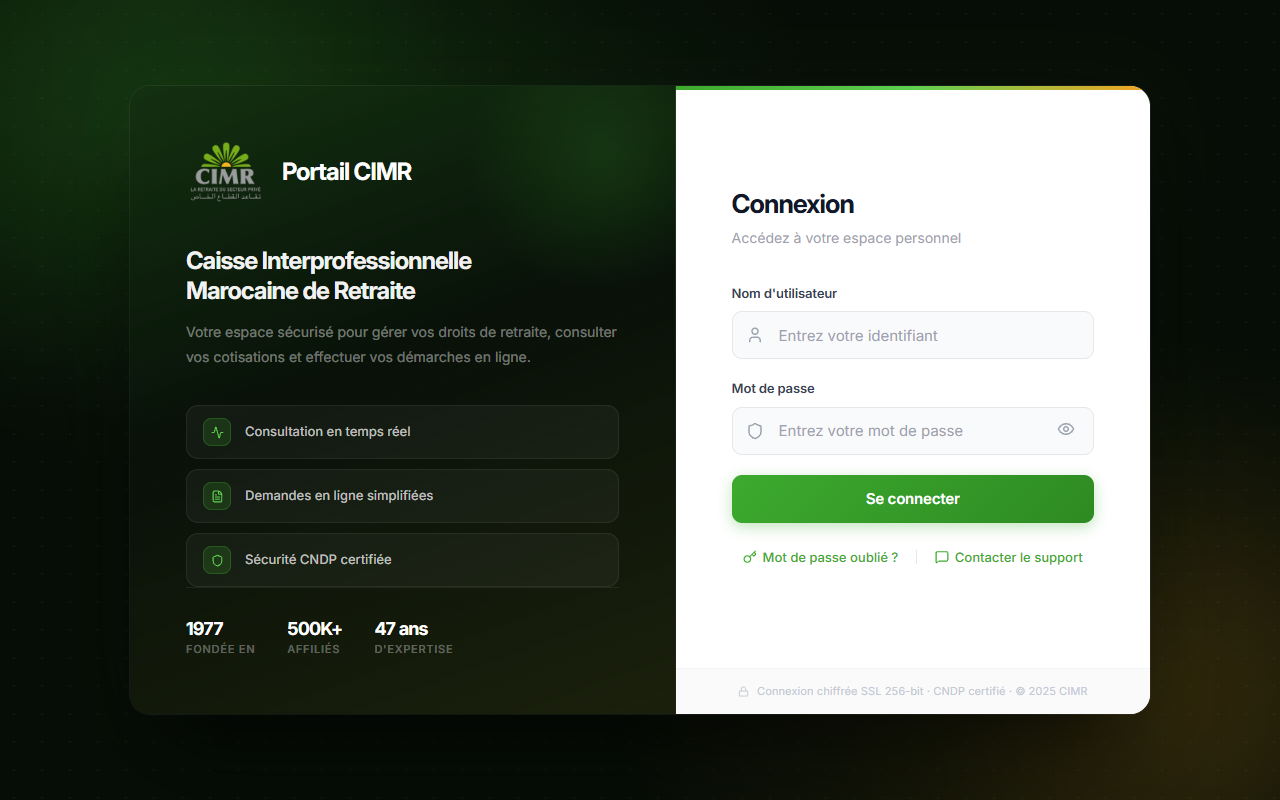
\includegraphics[width=0.85\textwidth]{captures/login.png}
\caption{Page de connexion}
\label{fig:login}
\end{figure}

\subsection{Réinitialisation de mot de passe}
Workflow en deux étapes : (1) saisie de l'e-mail $\to$ envoi d'un token, (2) saisie d'un nouveau mot de passe via le lien reçu. Le token est à durée limitée (15 minutes) et à usage unique.

\begin{figure}[H]
\centering
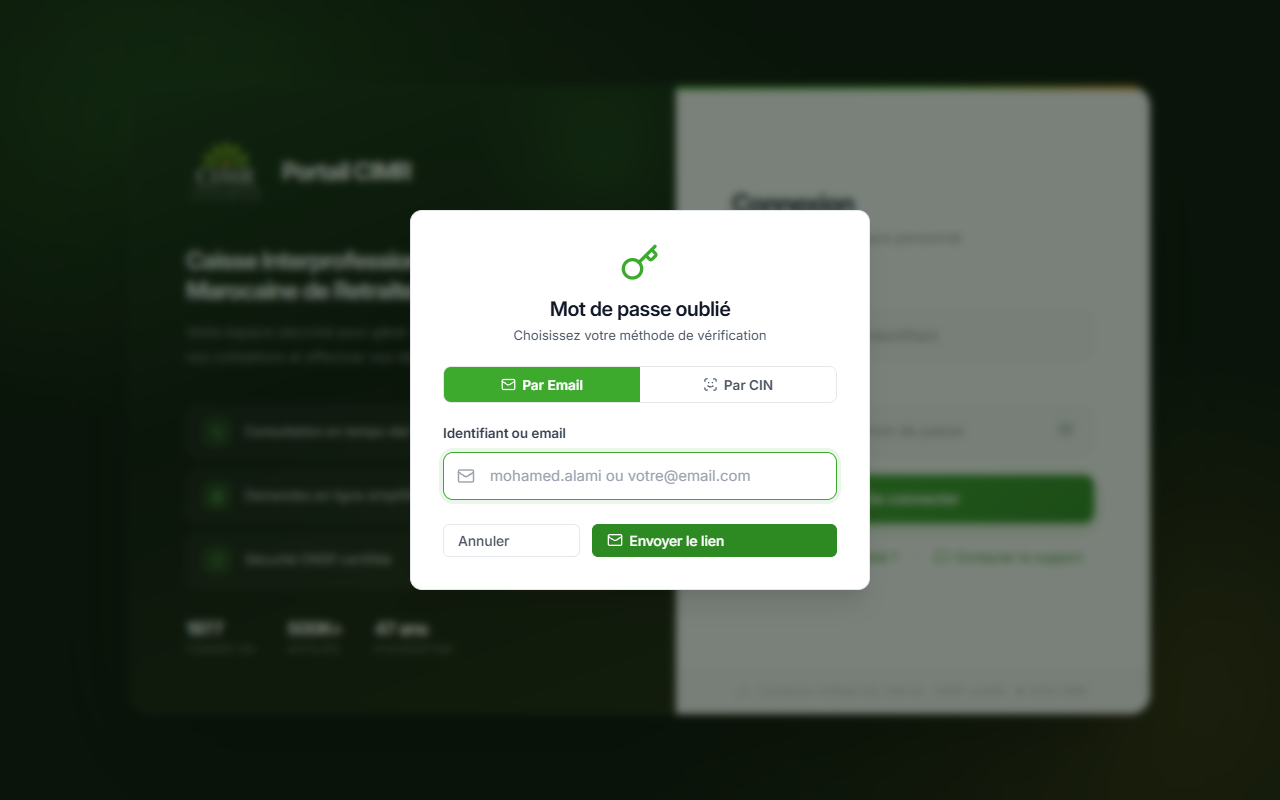
\includegraphics[width=0.85\textwidth]{captures/forgot_password.png}
\caption{Réinitialisation du mot de passe}
\end{figure}

\section{Tableau de bord}
Le tableau de bord est la première page consultée après connexion. Il agrège les informations clés selon le rôle de l'utilisateur :

\textbf{Pour un affilié :}
\begin{itemize}
    \item Nombre total de points cumulés (calculé à la volée) ;
    \item Estimation de la pension annuelle brute et nette ;
    \item Total des cotisations versées sur l'année ;
    \item Statut des dossiers en cours (liquidation, paiements) ;
    \item Cinq dernières notifications ;
    \item Liste des dossiers récents avec lien direct.
\end{itemize}

\textbf{Pour un administrateur :}
\begin{itemize}
    \item Nombre total d'affiliés actifs / radiés ;
    \item Volume des cotisations du mois ;
    \item Nombre de dossiers en attente d'instruction ;
    \item Graphique d'évolution des cotisations sur 12 mois.
\end{itemize}

\begin{figure}[H]
\centering
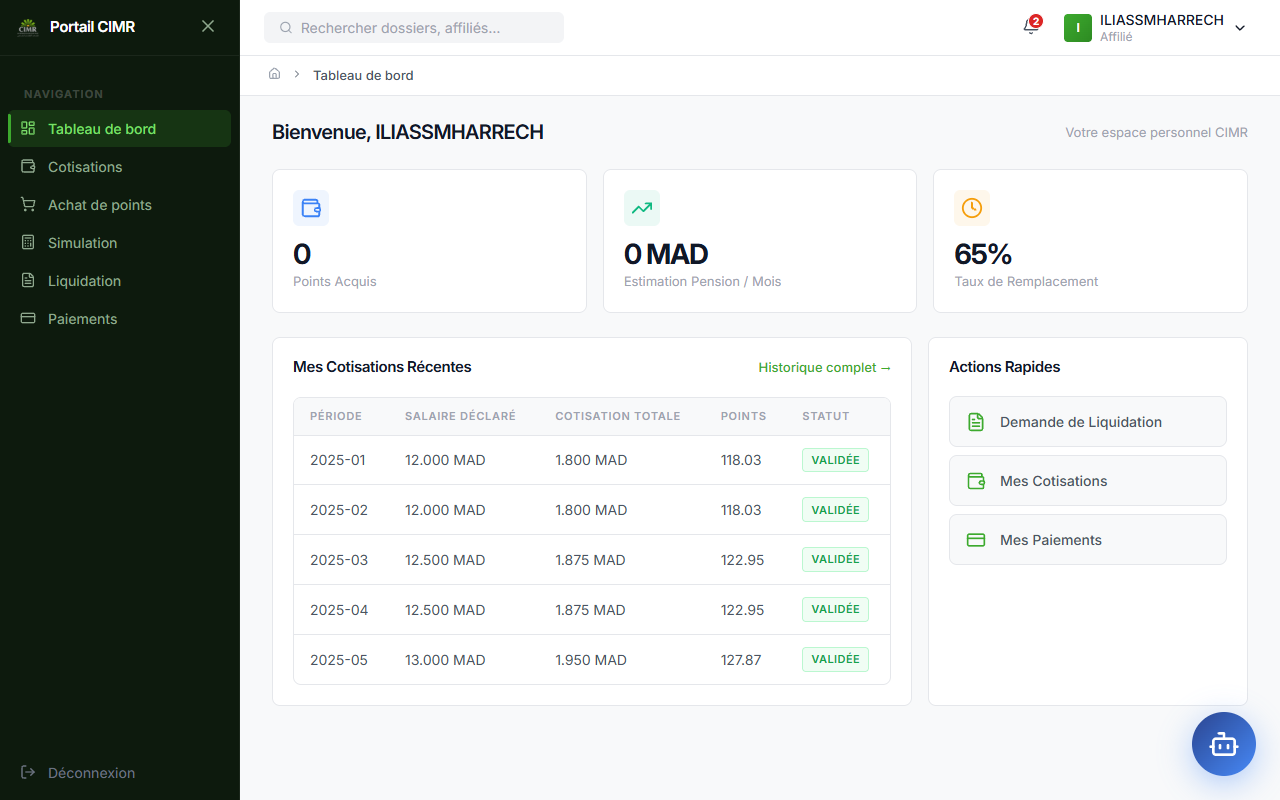
\includegraphics[width=0.85\textwidth]{captures/dashboard.png}
\caption{Tableau de bord affilié}
\label{fig:dashboard}
\end{figure}

\section{Module de simulation de pension}

\subsection{Présentation}
Le simulateur est l'une des fonctionnalités phares de la plateforme. Il permet à l'affilié d'estimer le montant de sa future pension selon différents scénarios. L'interface est structurée en \textbf{trois étapes (wizard)}.

\subsection{Étape 1 : Paramètres personnels}
Saisie du salaire mensuel actuel et de l'âge de départ souhaité (entre 55 et 70 ans).

\begin{figure}[H]
\centering
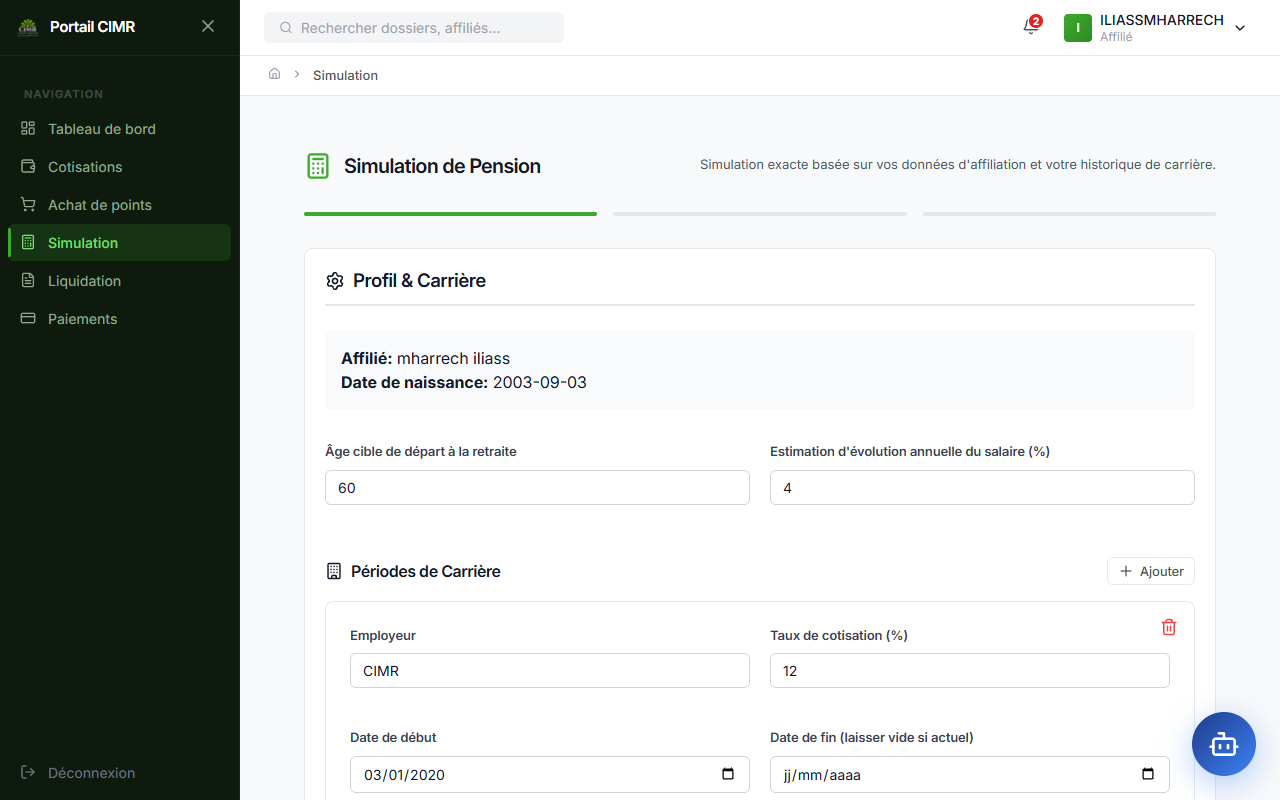
\includegraphics[width=0.85\textwidth]{captures/simulation_step1.png}
\caption{Simulation -- Étape 1 : Paramètres personnels}
\end{figure}

\subsection{Étape 2 : Options de rachat}
L'affilié peut choisir d'acheter des points supplémentaires pour augmenter sa future pension. Le calcul de l'impact est instantané.

\begin{figure}[H]
\centering
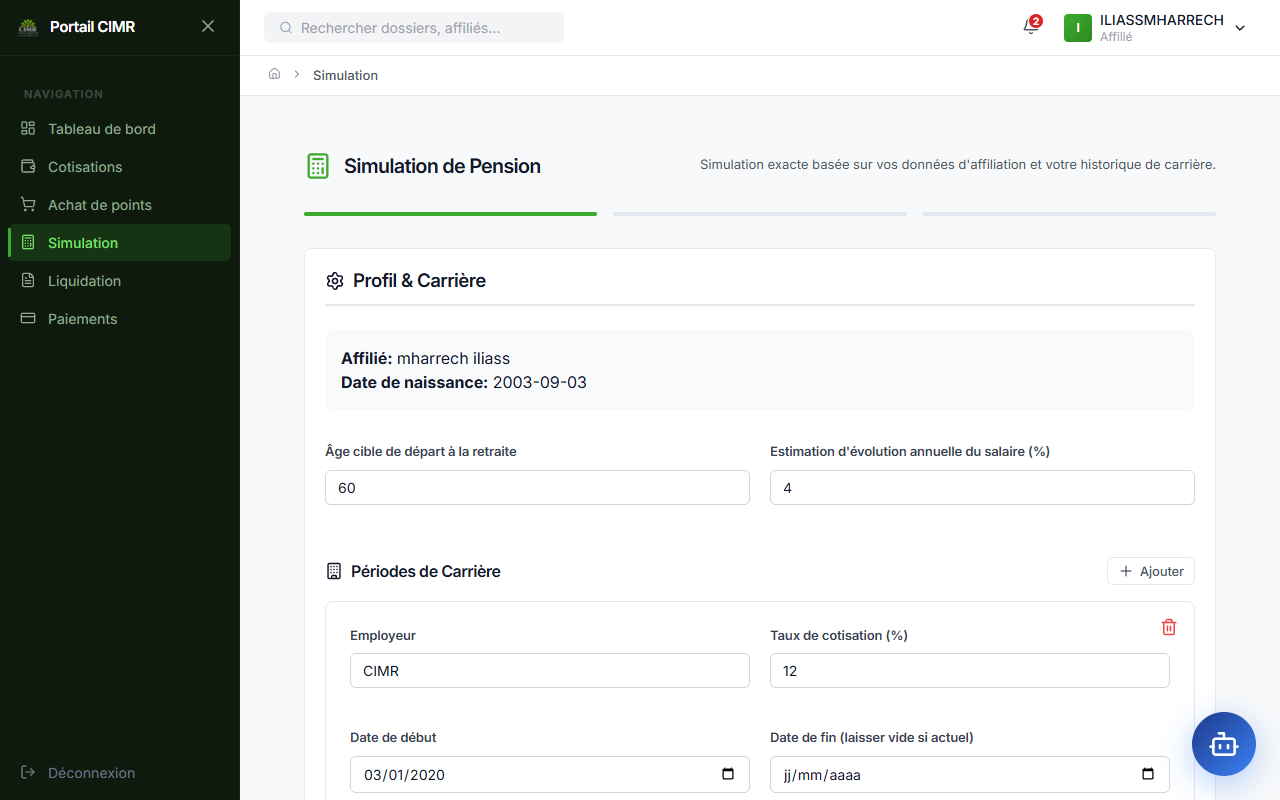
\includegraphics[width=0.85\textwidth]{captures/simulation_step2.png}
\caption{Simulation -- Étape 2 : Rachat de points}
\end{figure}

\subsection{Étape 3 : Résultat de la simulation}
Affichage du résultat final avec :
\begin{itemize}
    \item Pension annuelle brute et nette ;
    \item Évolution graphique des points sur la carrière ;
    \item Tableau comparatif de plusieurs scénarios ;
    \item Bouton d'export PDF du rapport de simulation.
\end{itemize}

Une validation côté frontend empêche l'affichage du résultat si la réponse backend est incomplète :

\begin{lstlisting}[language=Java,caption={Validation du résultat de simulation}]
if (!res?.summaryNet || !res?.summaryGross
    || !res?.careerSummaries || !res?.detailedProjections) {
  toast.error('Résultat de simulation incomplet. Vérifiez vos paramètres.');
  return;
}
setResults(res);
setStep(3);
\end{lstlisting}

\begin{figure}[H]
\centering
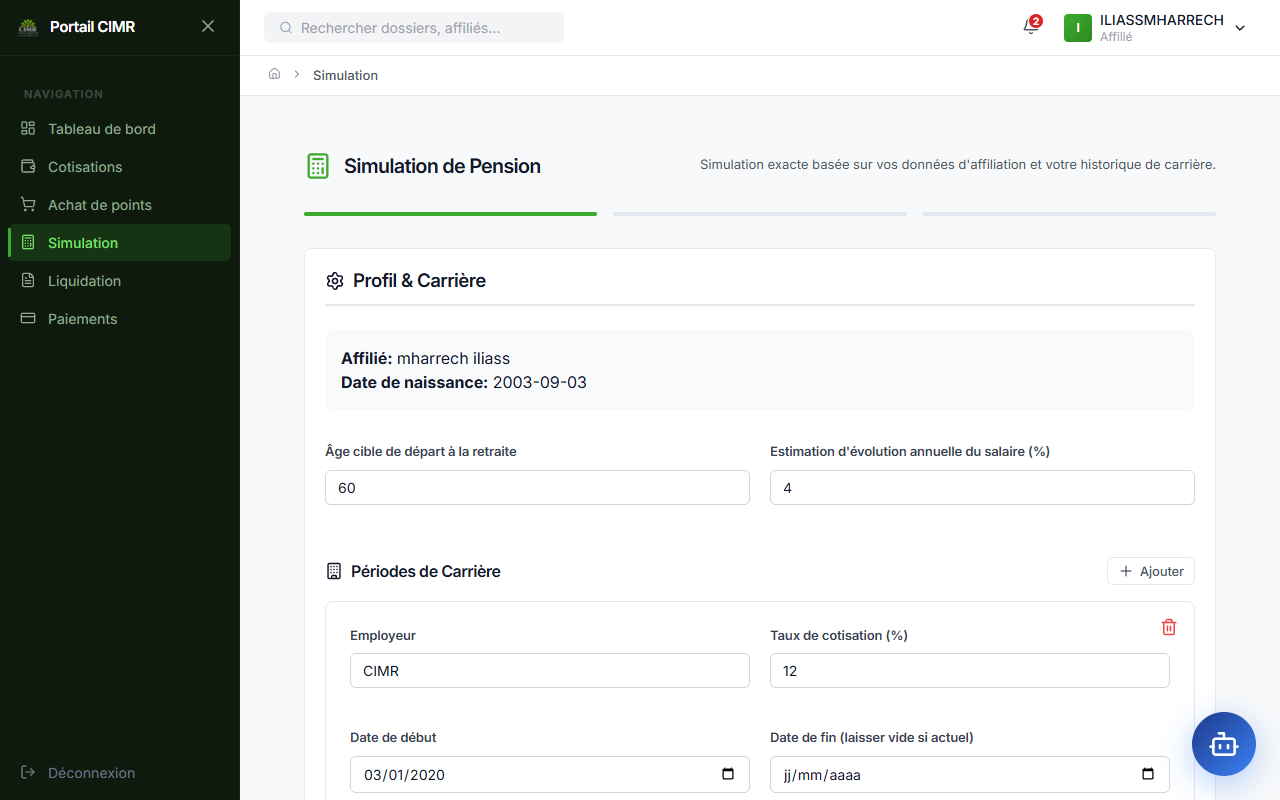
\includegraphics[width=0.85\textwidth]{captures/simulation_result.png}
\caption{Simulation -- Étape 3 : Résultat}
\label{fig:simulation}
\end{figure}

\section{Module de cotisations}

\subsection{Liste des cotisations}
Présentation paginée et triable de l'historique des cotisations mensuelles. Filtres disponibles : année, période, statut. Exports CSV et PDF disponibles.

\begin{figure}[H]
\centering
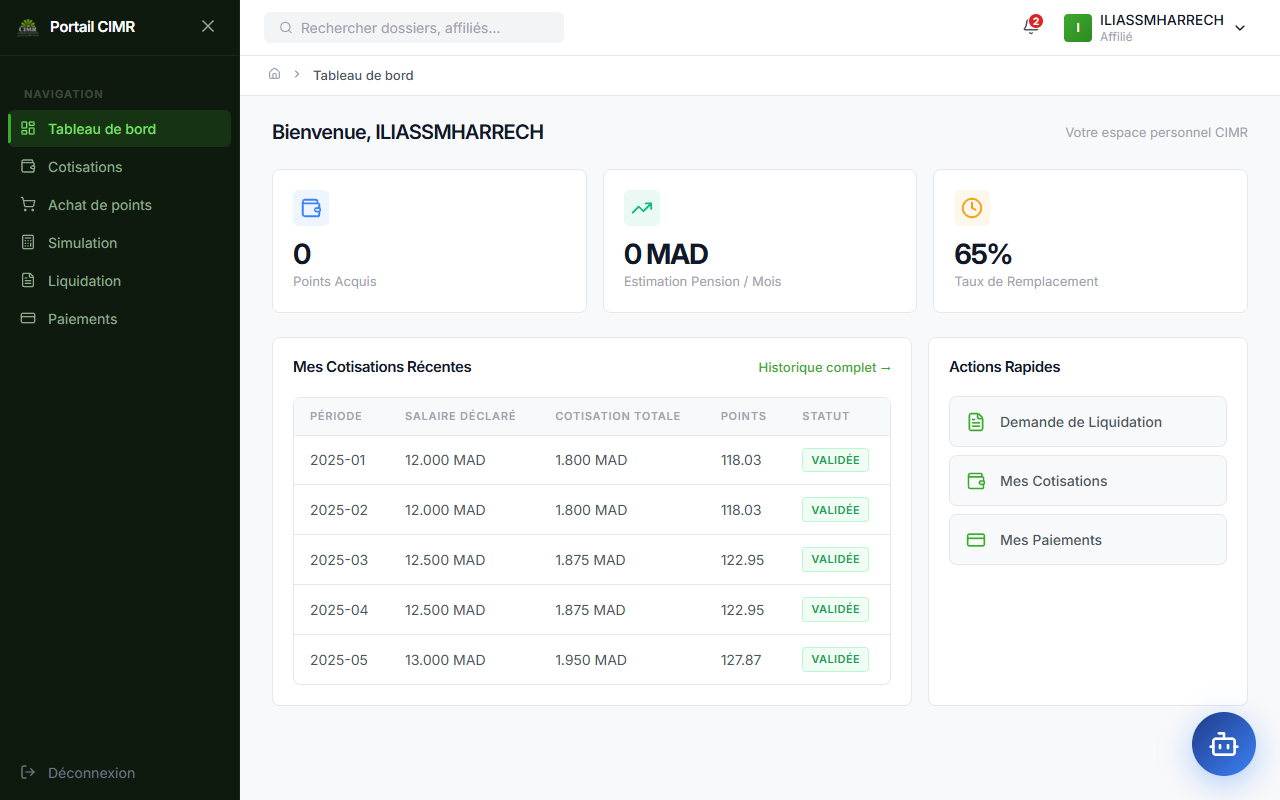
\includegraphics[width=0.85\textwidth]{captures/cotisations.png}
\caption{Page de la liste des cotisations}
\end{figure}

\subsection{Achat de points complémentaires}
Interface permettant à l'affilié d'acheter des points supplémentaires. Calcul instantané du coût selon la valeur d'achat de l'année courante. Confirmation par modal avant validation.

\begin{figure}[H]
\centering
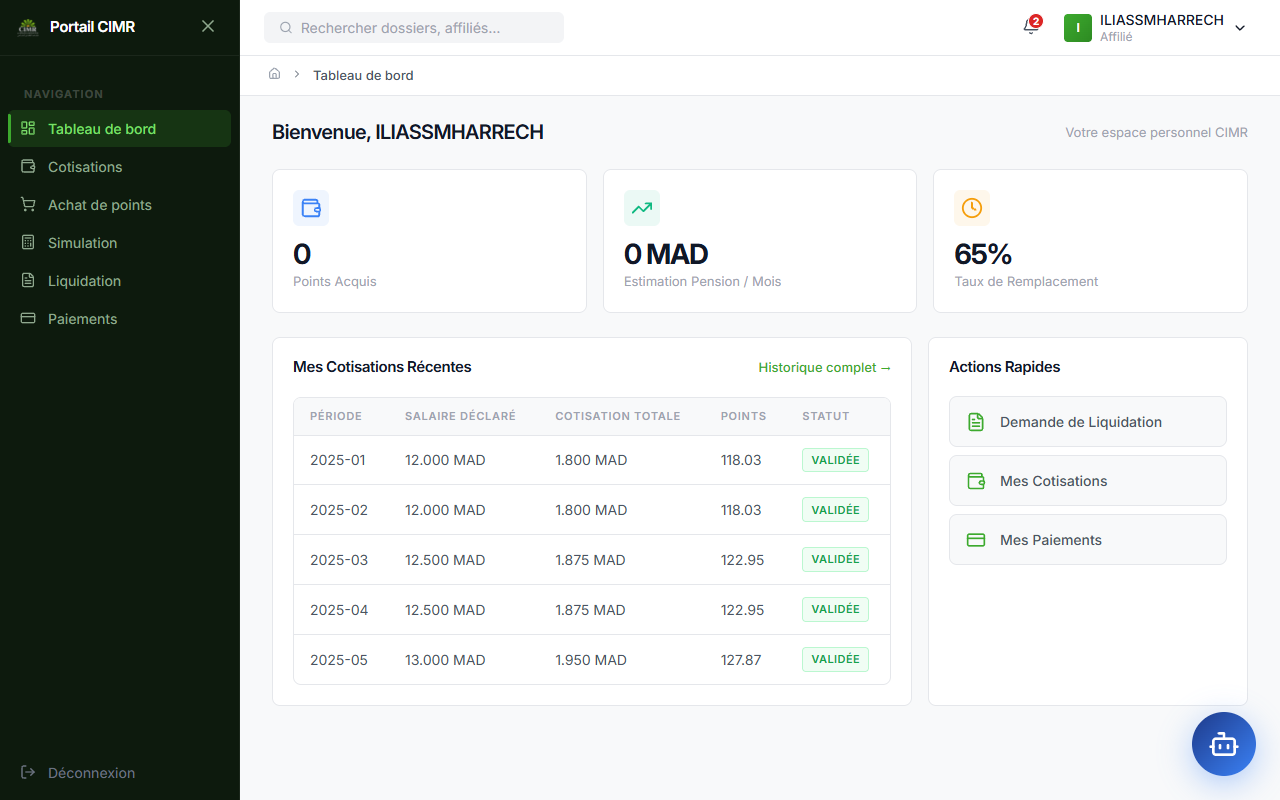
\includegraphics[width=0.85\textwidth]{captures/achat_points.png}
\caption{Page d'achat de points complémentaires}
\end{figure}

\section{Module de liquidation}

\subsection{Liste des demandes}
Vue principale du module liquidation : tableau listant toutes les demandes avec leurs statuts colorés (jaune = en attente, bleu = en cours, vert = validé, rouge = rejeté, gris = liquidé). Filtres par statut, date, affilié.

\begin{figure}[H]
\centering
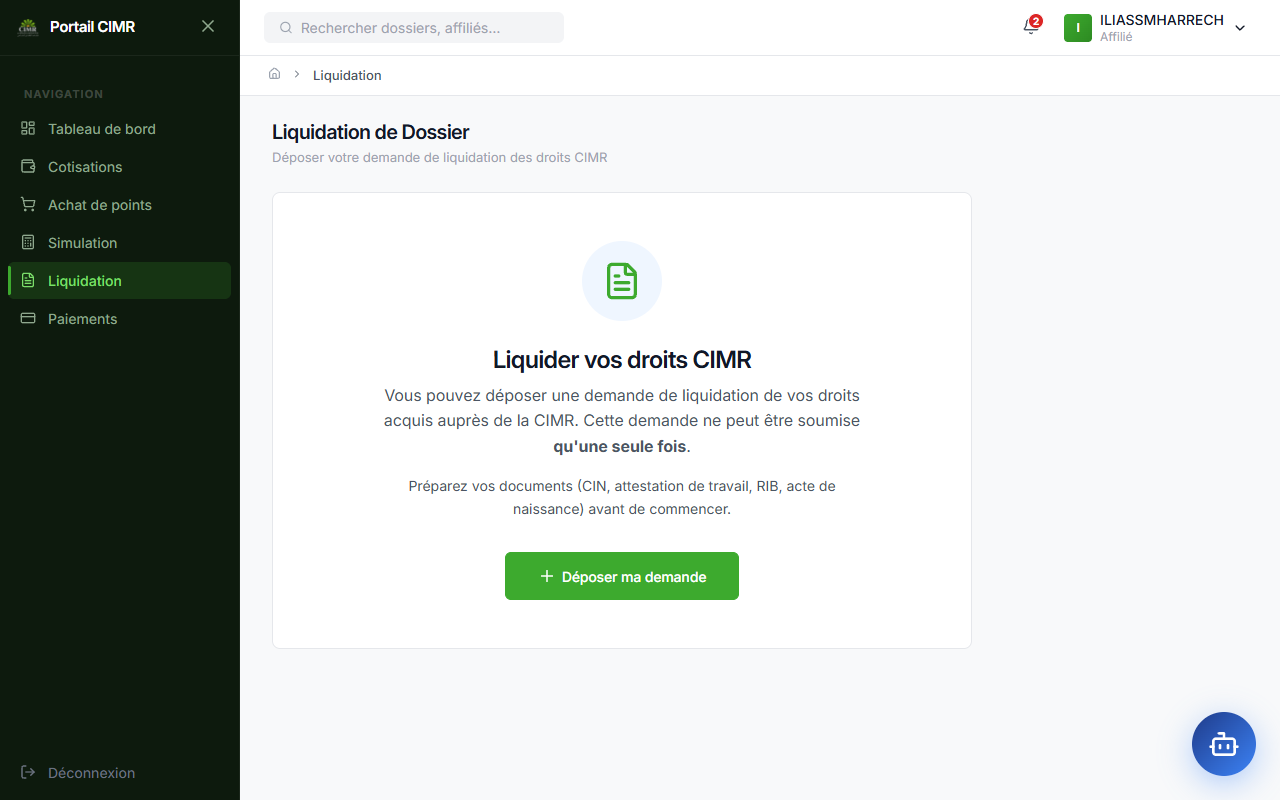
\includegraphics[width=0.85\textwidth]{captures/liste_liquidations.png}
\caption{Liste des demandes de liquidation}
\end{figure}

\subsection{Formulaire de nouvelle demande}
Formulaire structuré demandant : date d'effet souhaitée, type de liquidation (normale, anticipée), mode de paiement (virement, chèque), RIB, et téléversement des pièces justificatives obligatoires (CIN, RIB, certificat de cessation d'activité).

\begin{figure}[H]
\centering
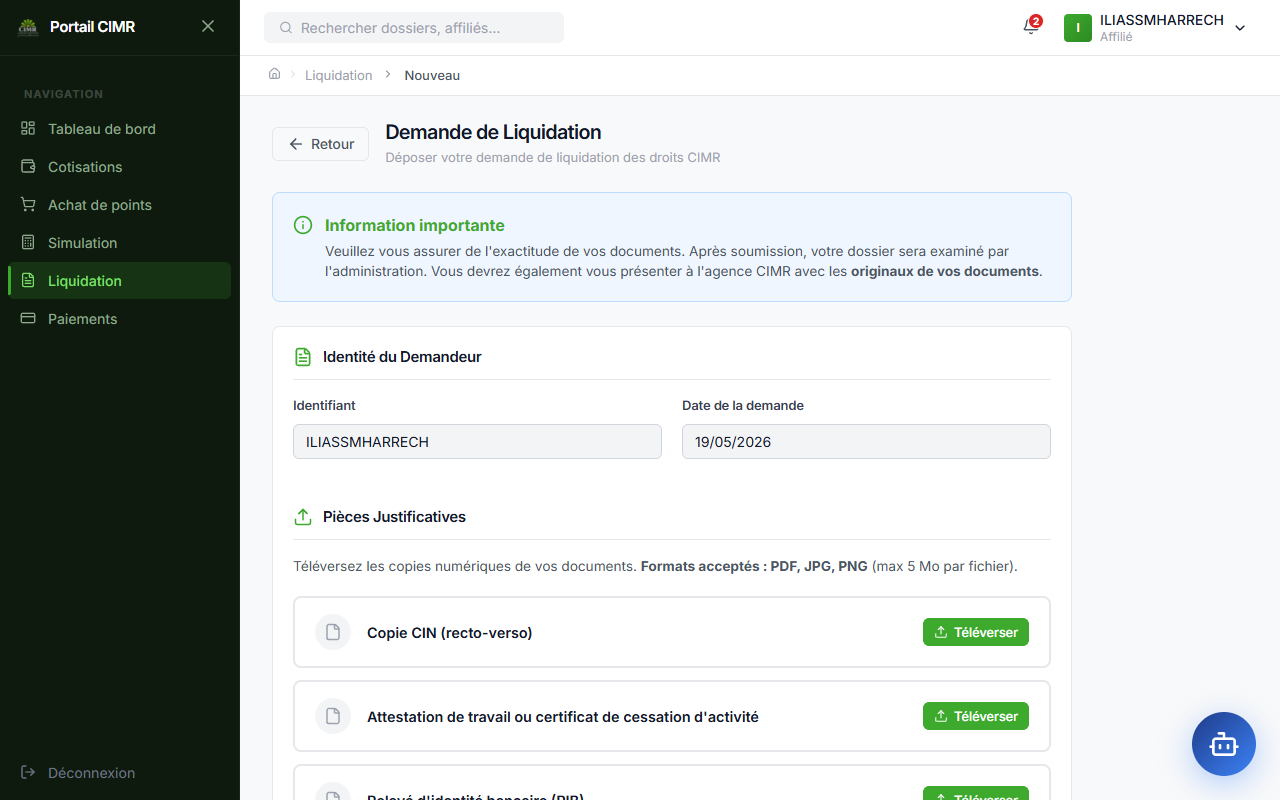
\includegraphics[width=0.85\textwidth]{captures/liquidation.png}
\caption{Formulaire de nouvelle demande de liquidation}
\label{fig:liquidation}
\end{figure}

\subsection{Workflow d'instruction (vue agent)}
Vue dédiée à l'agent CIMR permettant de changer le statut d'une demande. Le passage au statut \texttt{REJETE} impose la saisie obligatoire d'un \textbf{motif de rejet}, qui sera communiqué à l'affilié via notification.

\begin{figure}[H]
\centering
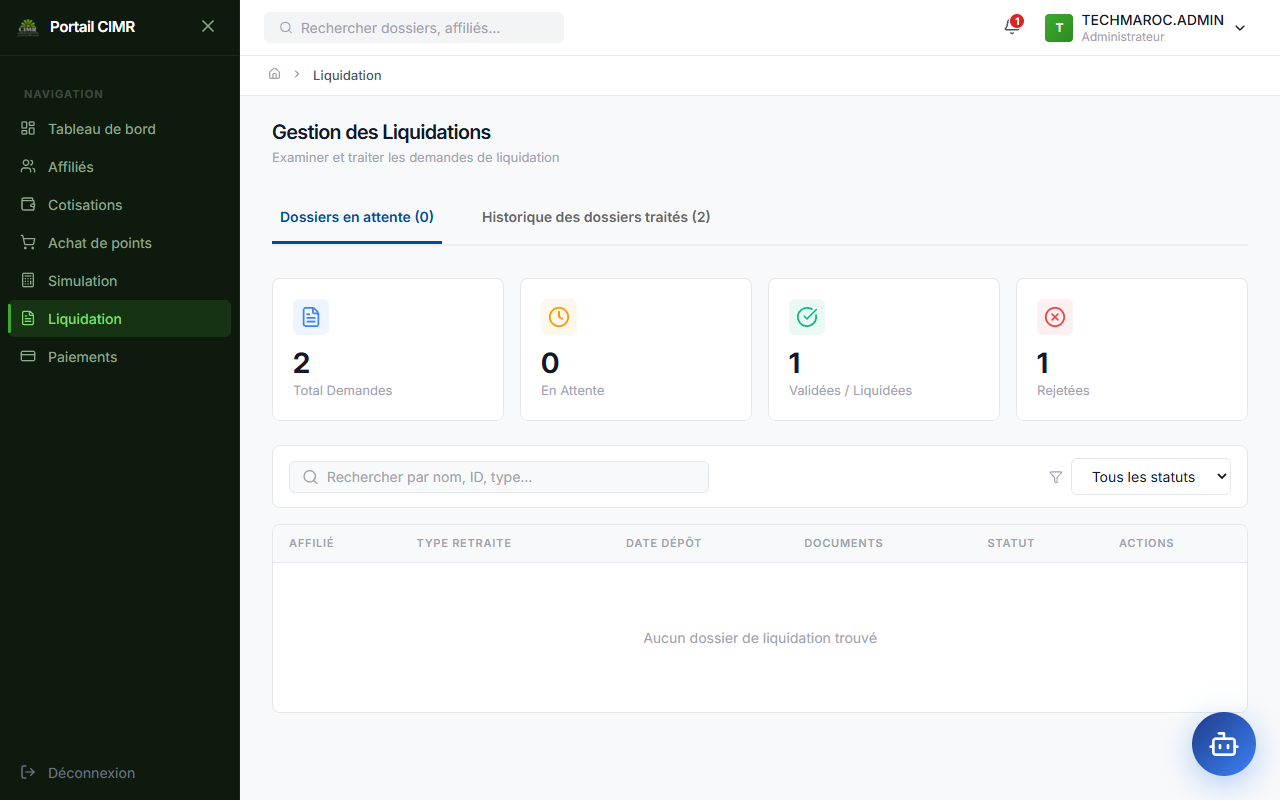
\includegraphics[width=0.85\textwidth]{captures/changement_statut.png}
\caption{Modal de changement de statut (vue agent)}
\end{figure}

\section{Module de paiements}

\subsection{Allocations}
Création et suivi des allocations (pension mensuelle, prime de fin d'année, etc.). Statuts gérés : \texttt{ACTIVE}, \texttt{SUSPENDED}, \texttt{TERMINATED}.

\begin{figure}[H]
\centering
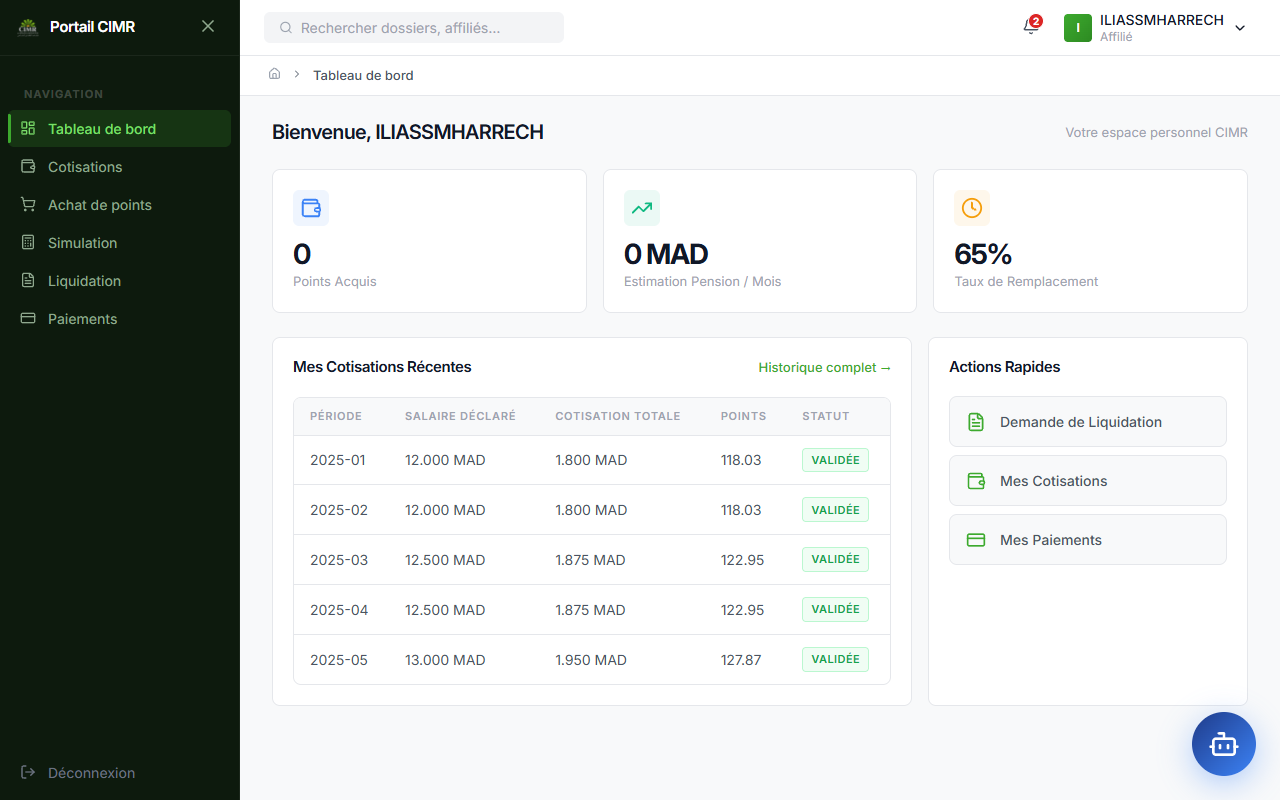
\includegraphics[width=0.85\textwidth]{captures/allocations.png}
\caption{Liste des allocations}
\end{figure}

\subsection{Programmation des paiements}
Modal de création d'un paiement : choix de l'allocation associée, montant, date, mode (virement / chèque). Réinitialisation automatique des formulaires sur succès ou fermeture.

\section{Module de réversion}

Module dédié à la gestion des pensions versées aux ayants droit d'un affilié décédé. Permet :
\begin{itemize}
    \item Déclaration du décès avec date et motif ;
    \item Enregistrement des ayants droit (conjoint, enfants orphelins) ;
    \item Calcul automatique du taux de réversion (50 \% conjoint, 25 \% par enfant orphelin) ;
    \item Workflow de validation avec gestion obligatoire du motif de rejet.
\end{itemize}

\begin{figure}[H]
\centering
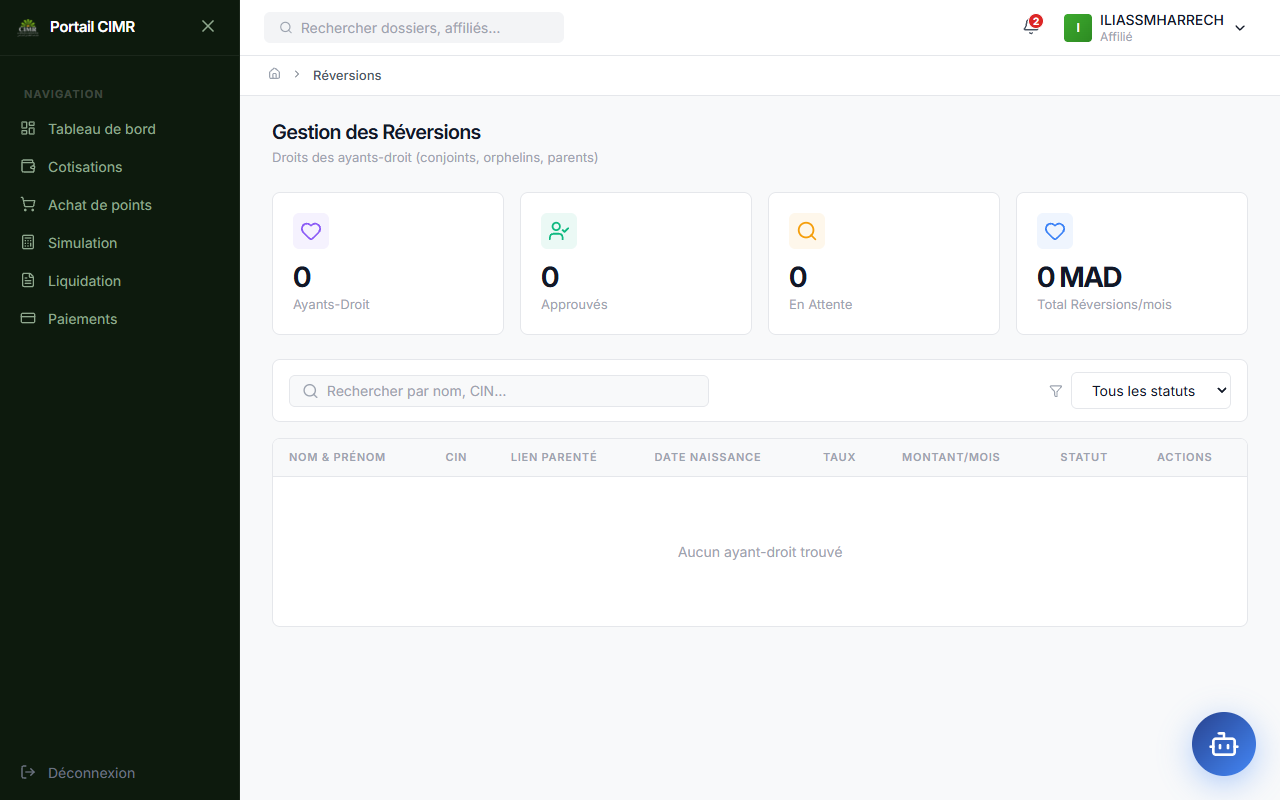
\includegraphics[width=0.85\textwidth]{captures/reversions.png}
\caption{Liste des dossiers de réversion}
\end{figure}

\section{Module de notifications}

Système de notifications en temps réel basé sur un \textbf{polling} (TanStack Query refetch toutes les 30 secondes) et alimenté côté backend par des \textbf{événements Kafka} consommés par \texttt{admin-service}. Chaque notification possède un type (info, succès, alerte, erreur), une date, un message et un éventuel lien contextuel.

\begin{figure}[H]
\centering
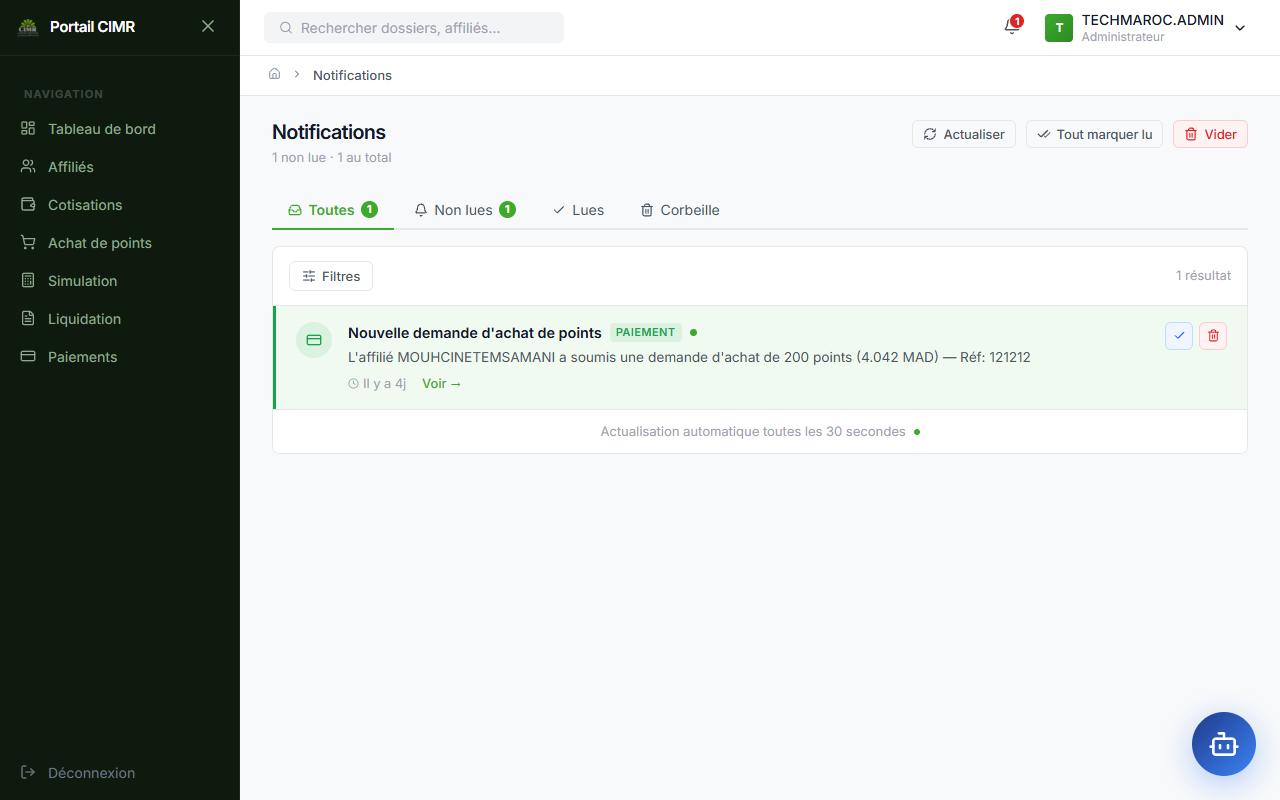
\includegraphics[width=0.85\textwidth]{captures/notifications.png}
\caption{Page des notifications}
\end{figure}

\section{Module d'audit (vue administrateur)}

\subsection{Journal d'audit}
Conformément à la \textbf{loi 09-08} (CNDP), toutes les actions sensibles (connexions, modifications de statut, accès aux données personnelles, suppressions) sont enregistrées dans un journal d'audit immuable. L'interface permet à l'administrateur de consulter, filtrer et exporter ces traces.

Filtres disponibles : utilisateur, date, type d'action, ressource concernée.

\begin{figure}[H]
\centering
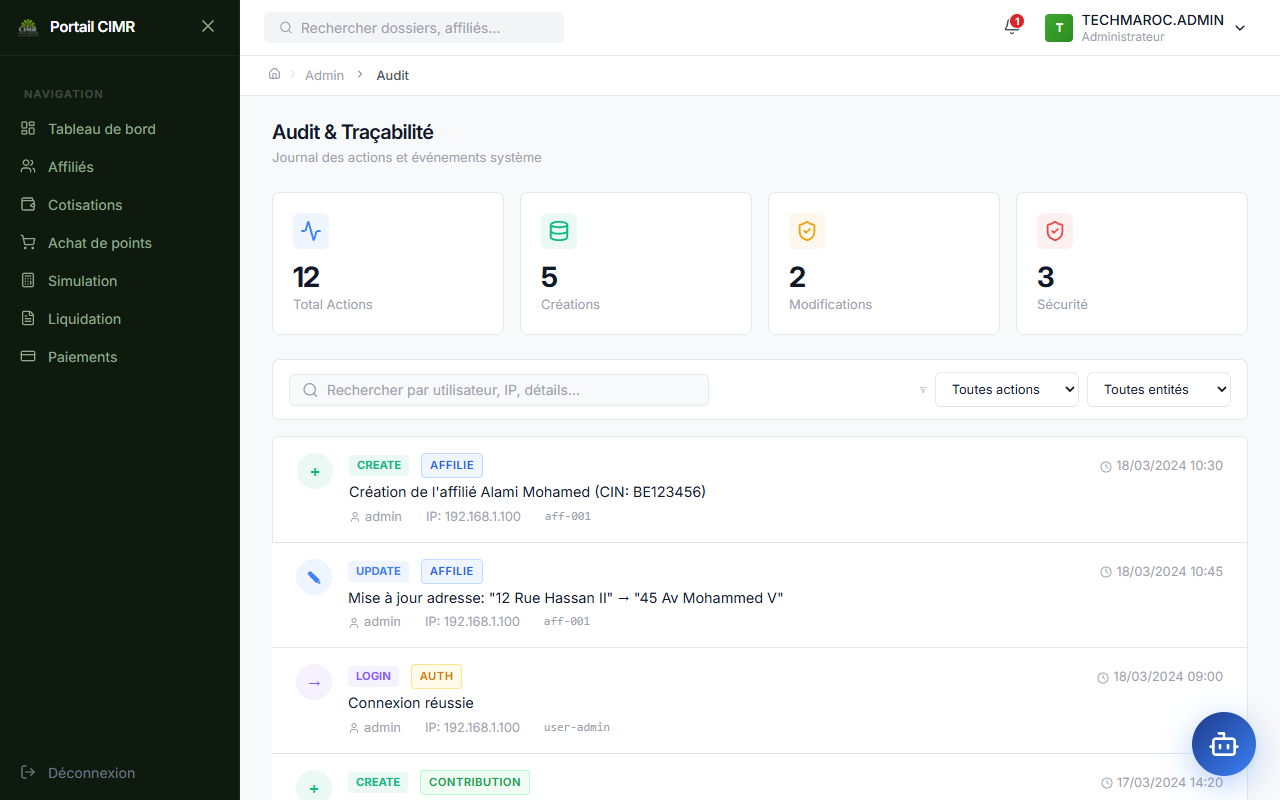
\includegraphics[width=0.85\textwidth]{captures/audit.png}
\caption{Journal d'audit (vue administrateur)}
\label{fig:audit}
\end{figure}

\section{Module de profil et paramètres}

Pages permettant à l'utilisateur de mettre à jour ses informations personnelles, son mot de passe et ses préférences (langue, notifications). Les modifications sensibles (mot de passe, email) déclenchent un événement d'audit.

\begin{figure}[H]
\centering
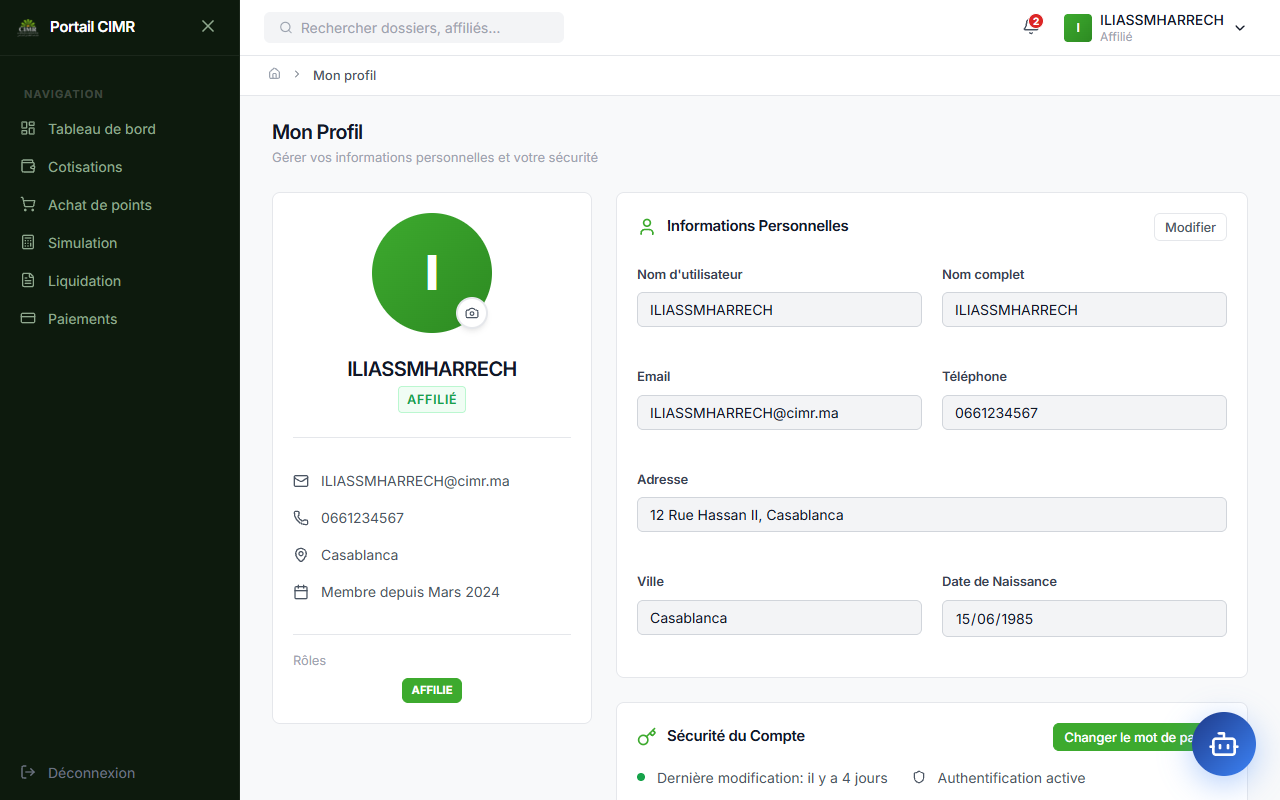
\includegraphics[width=0.85\textwidth]{captures/profile.png}
\caption{Page de profil utilisateur}
\end{figure}

\section{Synthèse des écrans livrés}

Au total, l'application livrée comprend \textbf{18 pages frontend} entièrement fonctionnelles et intégrées au backend :

\begin{table}[H]
\centering
\caption{Récapitulatif des écrans livrés}
\begin{tabular}{lll}
\toprule
\textbf{Module} & \textbf{Pages} & \textbf{État} \\
\midrule
Authentification & Login, Reset Password & Livré \\
Tableau de bord & Dashboard & Livré \\
Affiliation & Liste, Formulaire, Détail & Livré \\
Cotisations & Liste, Achat de points & Livré \\
Simulation & Wizard 3 étapes & Livré \\
Liquidation & Liste, Formulaire & Livré \\
Paiements & Liste, Modals & Livré \\
Réversion & Liste & Livré \\
Notifications & Liste, Détail & Livré \\
Audit (admin) & Journal & Livré \\
Profil / Paramètres & Profil, Settings & Livré \\
\bottomrule
\end{tabular}
\end{table}

\section{Conclusion}
Le développement a abouti à une application web complète, intégrée et fonctionnelle, couvrant l'intégralité du parcours utilisateur prévu dans la phase de conception. Les écrans réalisés respectent les principes d'ergonomie modernes (responsive, navigation intuitive, feedback utilisateur) et reposent sur une architecture technique solide. Le chapitre suivant détaille la démarche de tests qui a permis de valider la qualité de ces livrables.

% ============================================================
% CHAPITRE 7 - TESTS
% ============================================================
\chapter{Tests et Validation}

\section{Introduction}
Stratégie de tests garantissant la fiabilité du système.

\section{Stratégie de test}
Pyramide classique : nombreux tests unitaires, quelques tests d'intégration, peu de tests E2E.

\begin{table}[H]
\centering
\caption{Plan de tests}
\begin{tabular}{lll}
\toprule
\textbf{Niveau} & \textbf{Outils} & \textbf{Couverture} \\
\midrule
Unit. backend & JUnit 5, Mockito & \textgreater{} 70 \% \\
Unit. frontend & Vitest, RTL & \textgreater{} 60 \% \\
Intégration & Spring Test, Testcontainers & scénarios principaux \\
API & Postman & toutes routes \\
E2E & Playwright manuel & parcours critiques \\
\bottomrule
\end{tabular}
\end{table}

\section{Tests unitaires backend}

\begin{lstlisting}[language=Java,caption={Exemple de test unitaire}]
@ExtendWith(MockitoExtension.class)
class PointValueServiceTest {

    @Mock private PointValueRepository repository;
    @InjectMocks private PointValueService service;

    @Test
    void shouldUpdateExistingPointValueForYear() {
        PointValue existing = new PointValue(2025, BigDecimal.valueOf(15.0));
        when(repository.findByYear(2025)).thenReturn(Optional.of(existing));
        when(repository.save(any())).thenAnswer(i -> i.getArgument(0));

        PointValue input = new PointValue(2025, BigDecimal.valueOf(16.0));
        PointValue result = service.savePointValue(input);

        assertEquals(BigDecimal.valueOf(16.0), result.getValue());
        verify(repository).save(existing);
    }
}
\end{lstlisting}

\section{Tests d'intégration}
Avec \textbf{Testcontainers} : vraie instance PostgreSQL le temps du test.

\section{Tests d'API (Postman)}
Collection couvrant : authentification, CRUD affiliés, cycle de liquidation.

\section{Tests utilisateurs}
Session avec 5 personnes. Scénarios : connexion, simulation, liquidation, notifications.

\textbf{Retours :}
\begin{itemize}
    \item Interface jugée claire et moderne ;
    \item Simulateur très apprécié ;
    \item Souhait de plus d'icônes explicatives ;
    \item Demande de tutoriel d'accueil.
\end{itemize}

\section{Résultats}
\begin{table}[H]
\centering
\caption{Résultats des tests}
\begin{tabular}{lr}
\toprule
\textbf{Indicateur} & \textbf{Valeur} \\
\midrule
Tests unitaires backend & 120 \\
Tests unitaires frontend & 45 \\
Couverture moyenne backend & 65 \% \\
Bugs détectés et corrigés & 28 \\
Bugs critiques résolus & 100 \% \\
\bottomrule
\end{tabular}
\end{table}

\section{Conclusion}
Niveau de qualité satisfaisant pour un projet académique. Perspectives : augmenter la couverture, tests de performance JMeter, automatisation E2E en CI/CD.

% ============================================================
% CHAPITRE 7 - DÉPLOIEMENT
% ============================================================
\chapter{Déploiement}

\section{Introduction}
Architecture, procédures, configuration et maintenance.

\section{Architecture de déploiement}
\textbf{Docker Compose} orchestre 12 conteneurs : 9 microservices + PostgreSQL + Kafka + Zookeeper.

\section{Configuration requise}

\subsection{Matériel}
\begin{table}[H]
\centering
\begin{tabular}{lll}
\toprule
\textbf{Ressource} & \textbf{Minimum} & \textbf{Recommandé} \\
\midrule
CPU & 4 cœurs & 8 cœurs \\
RAM & 8 GB & 16 GB \\
Disque & 20 GB SSD & 50 GB SSD \\
\bottomrule
\end{tabular}
\end{table}

\subsection{Logiciels prérequis}
\begin{itemize}
    \item Docker Desktop 4.30+ ou Docker Engine 24+
    \item Git 2.40+
    \item Node.js 20 LTS (dev frontend)
\end{itemize}

\section{Procédure d'installation}

\textbf{Étape 1 --- Clonage}
\begin{lstlisting}[language=bash]
git clone https://github.com/marwane3214/projet-fin-d-etude.git
cd projet-fin-d-etude-main
\end{lstlisting}

\textbf{Étape 2 --- Build}
\begin{lstlisting}[language=bash]
cd backend
docker compose build
\end{lstlisting}

\textbf{Étape 3 --- Démarrage}
\begin{lstlisting}[language=bash]
docker compose up -d
docker compose ps
\end{lstlisting}

\textbf{Étape 4 --- Frontend}
\begin{lstlisting}[language=bash]
cd ../frontend
npm install
npm run dev
\end{lstlisting}

Accès : \texttt{http://localhost:5173}

\section{Comptes de test}
\begin{table}[H]
\centering
\caption{Comptes de démonstration}
\begin{tabular}{lll}
\toprule
\textbf{Email} & \textbf{Mot de passe} & \textbf{Rôle} \\
\midrule
admin@cimr.ma & Admin@2025 & ADMIN \\
agent@cimr.ma & Agent@2025 & AGENT \\
affilie@cimr.ma & Affilie@2025 & AFFILIE \\
\bottomrule
\end{tabular}
\end{table}

\section{Maintenance}
\begin{itemize}
    \item Sauvegardes : \texttt{pg\_dump} quotidien.
    \item Mises à jour : rolling update via Docker Compose.
    \item Monitoring : Actuator endpoints (\texttt{/actuator/health}, \texttt{/actuator/metrics}).
\end{itemize}

\section{Conclusion}
Docker Compose offre une solution simple, reproductible, portable. Pour la production : Kubernetes (EKS, AKS, GKE).

% ============================================================
% CHAPITRE 8 - GUIDE UTILISATEUR
% ============================================================
\chapter{Guide Utilisateur}

\section{Introduction}
Usage pas à pas des fonctionnalités principales.

\section{Première connexion}
\begin{enumerate}
    \item Ouvrir \texttt{http://localhost:5173}.
    \item Saisir email + mot de passe.
    \item Cliquer sur « Se connecter ».
\end{enumerate}

\section{Tableau de bord}
Affichage des points cumulés, estimation pension, historique cotisations, statut des dossiers et notifications.

\section{Simuler sa pension}
\begin{enumerate}
    \item Menu « Simulation ».
    \item Étape 1 : salaire mensuel + âge de départ (55-70 ans).
    \item Étape 2 : rachat éventuel de points.
    \item Étape 3 : visualisation du résultat (brut, net, scénarios).
    \item Export PDF possible.
\end{enumerate}

\section{Déposer une demande de liquidation}
\begin{enumerate}
    \item Menu « Liquidations » \textgreater{} « Nouvelle demande ».
    \item Remplir le formulaire (date d'effet, mode paiement, RIB).
    \item Téléverser : CIN, RIB, certificat de cessation d'activité.
    \item Soumettre. Un numéro de dossier est attribué.
\end{enumerate}

\section{Consulter ses cotisations}
Menu « Cotisations » : liste paginée avec période, salaire, montant, points. Export CSV / PDF.

\section{Acheter des points}
Menu « Points complémentaires » \textgreater{} sélection du nombre de points \textgreater{} affichage du coût \textgreater{} paiement.

\section{Notifications}
Cloche en haut à droite. Au clic : liste des notifications (type, date, message, lien).

\section{FAQ}
\textbf{Connexion impossible ?} Vérifier email et mot de passe ; sinon « Mot de passe oublié ».

\textbf{Upload refusé ?} Format PDF/JPG/PNG, taille \textless{} 10 Mo.

\textbf{Simulation incohérente ?} Vérifier les valeurs (salaire MAD, années entières).

\section{Conclusion}
Interface accessible, iconographie claire, parcours linéaires.

% ============================================================
% CONCLUSION GÉNÉRALE
% ============================================================
\chapter*{Conclusion et Perspectives}
\addcontentsline{toc}{chapter}{Conclusion et Perspectives}

\section*{Synthèse du travail réalisé}
Ce PFA a permis de \textbf{concevoir, développer et déployer une plateforme digitale complète de gestion des retraites} inspirée du contexte de la CIMR. Le travail couvre l'intégralité du cycle d'un projet logiciel professionnel : analyse, conception, développement, tests, déploiement, documentation.

Au total : \textbf{9 microservices backend}, \textbf{18 pages frontend}, \textbf{7 bases de données}.

\section*{Évaluation des objectifs}
\begin{table}[H]
\centering
\begin{tabular}{lll}
\toprule
\textbf{Objectif} & \textbf{Statut} & \textbf{Commentaire} \\
\midrule
O1 Architecture microservices & Atteint & 9 services autonomes \\
O2 Plateforme web complète & Atteint & 18 pages responsive \\
O3 Moteur de simulation & Atteint & Multi-scénarios + Zod \\
O4 Workflow liquidation & Atteint & 6 statuts, GED \\
O5 Sécurité et conformité & Atteint & JWT, chiffrement, audit \\
O6 Communication asynchrone & Atteint & Kafka audit/notif \\
O7 Conteneurisation & Atteint & Docker Compose 12 \\
\bottomrule
\end{tabular}
\end{table}

\section*{Limitations actuelles}
\begin{itemize}
    \item Pas de déploiement cloud (local Docker Compose).
    \item Couverture de tests partielle ($\sim$65 \%).
    \item Données simulées (pas d'intégration externe réelle).
    \item Pas d'application mobile native.
    \item Mono-langue (français).
\end{itemize}

\section*{Perspectives d'évolution}

\textbf{Court terme :}
\begin{itemize}
    \item Couverture de tests \textgreater{} 85 \%.
    \item Internationalisation (arabe, anglais).
    \item Mode sombre.
    \item Optimisations (lazy loading, code splitting).
\end{itemize}

\textbf{Moyen terme :}
\begin{itemize}
    \item Migration Kubernetes (EKS).
    \item CI/CD GitLab/GitHub Actions.
    \item Monitoring Prometheus + Grafana + ELK.
    \item Application mobile (React Native / Flutter).
    \item Signature électronique.
\end{itemize}

\textbf{Long terme :}
\begin{itemize}
    \item IA : détection de fraude, recommandation départ retraite.
    \item Blockchain pour traçabilité immuable.
    \item Interconnexion CNSS, banques, administrations.
    \item Chatbot LLM.
    \item Open Banking.
\end{itemize}

\section*{Mot final}
Au-delà d'un livrable technique, ce projet est une \textbf{expérience de transformation digitale} appliquée à un secteur stratégique pour le Maroc. Les compétences acquises constituent un capital précieux pour la suite du parcours académique et professionnel et posent les fondations d'une éventuelle évolution en PFE ou en startup FinTech.

% ============================================================
% RÉFÉRENCES
% ============================================================
\chapter*{Références}
\addcontentsline{toc}{chapter}{Références}

\subsection*{Ouvrages}
\begin{enumerate}
    \item Newman, S. (2021). \textit{Building Microservices: Designing Fine-Grained Systems} (2nd ed.). O'Reilly Media.
    \item Richardson, C. (2018). \textit{Microservices Patterns: With Examples in Java}. Manning.
    \item Walls, C. (2022). \textit{Spring in Action} (6th ed.). Manning.
    \item Banks, A., \& Porcello, E. (2020). \textit{Learning React} (2nd ed.). O'Reilly Media.
    \item Kleppmann, M. (2017). \textit{Designing Data-Intensive Applications}. O'Reilly.
\end{enumerate}

\subsection*{Documentations officielles}
\begin{enumerate}\setcounter{enumi}{5}
    \item Spring Boot Documentation --- \url{https://docs.spring.io/spring-boot/}
    \item Spring Cloud Gateway --- \url{https://docs.spring.io/spring-cloud-gateway/}
    \item React Documentation --- \url{https://react.dev/}
    \item TypeScript Handbook --- \url{https://www.typescriptlang.org/docs/}
    \item PostgreSQL 15 --- \url{https://www.postgresql.org/docs/15/}
    \item Apache Kafka --- \url{https://kafka.apache.org/documentation/}
    \item Docker Documentation --- \url{https://docs.docker.com/}
    \item TanStack Query --- \url{https://tanstack.com/query/latest}
    \item Tailwind CSS --- \url{https://tailwindcss.com/docs}
\end{enumerate}

\subsection*{Réglementation}
\begin{enumerate}\setcounter{enumi}{14}
    \item Loi n° 09-08 relative à la protection des données --- Royaume du Maroc.
    \item Commission Nationale CNDP --- \url{https://www.cndp.ma}
    \item RFC 7519 : JSON Web Token (JWT) --- IETF.
    \item OWASP Top 10 (2021) --- \url{https://owasp.org/Top10/}
\end{enumerate}

\subsection*{Contexte CIMR}
\begin{enumerate}\setcounter{enumi}{18}
    \item CIMR --- Site officiel --- \url{https://www.cimr.ma}
    \item Rapport annuel CIMR 2023.
\end{enumerate}

% ============================================================
% ANNEXES
% ============================================================
\appendix
\chapter{Annexes}

\section{Exemple d'endpoint REST documenté}
\begin{lstlisting}[language=Java]
@RestController
@RequestMapping("/api/liquidations")
@Tag(name = "Liquidations")
public class LiquidationController {

    @Operation(summary = "Créer une demande de liquidation")
    @ApiResponse(responseCode = "201", description = "Créée")
    @PostMapping
    public ResponseEntity<DemandeLiquidationDTO> create(
            @Valid @RequestBody CreateLiquidationRequest request) {
        var saved = service.create(request);
        return ResponseEntity.status(HttpStatus.CREATED)
                             .body(mapper.toDto(saved));
    }
}
\end{lstlisting}

\section{Extrait de docker-compose.yml}
\begin{lstlisting}[language=bash]
version: '3.9'
services:
  postgres:
    image: postgres:15
    environment:
      POSTGRES_USER: cimr
      POSTGRES_PASSWORD: cimr_secret_2024
    ports: ["5435:5432"]
    networks: [cimr-network]

  kafka:
    image: confluentinc/cp-kafka:7.5.3
    ports: ["9092:9092"]
    depends_on: [zookeeper]

  auth-service:
    build:
      context: .
      dockerfile: auth-service/Dockerfile
    ports: ["8079:8079"]
    environment:
      SPRING_DATASOURCE_URL: jdbc:postgresql://postgres:5432/cimr_auth
    depends_on: [postgres]

networks:
  cimr-network:
    driver: bridge
\end{lstlisting}

\section{Planification du projet (Gantt)}
\begin{lstlisting}
Semaine     1  2  3  4  5  6  7  8  9 10 11 12 13 14 15 16
Analyse    ===
Conception    ======
Backend           ================
Frontend             ===================
Intégration                       ======
Tests                                ========
Déploiement                              ====
Rapport                                     =========
\end{lstlisting}

\section{Dépendances frontend (package.json)}
\begin{lstlisting}[language=Java]
{
  "dependencies": {
    "react": "^19.2.4",
    "react-dom": "^19.2.4",
    "react-router-dom": "^7.13.1",
    "@tanstack/react-query": "^5.90.21",
    "axios": "^1.13.6",
    "react-hook-form": "^7.71.2",
    "zod": "^4.3.6",
    "framer-motion": "^12.38.0",
    "lucide-react": "^0.460.0",
    "tailwindcss": "^4.0.0"
  },
  "devDependencies": {
    "typescript": "^5.9.0",
    "vite": "^8.0.0",
    "@vitejs/plugin-react": "^4.3.0"
  }
}
\end{lstlisting}



\vspace{2cm}
\begin{center}
\textbf{--- Fin du document ---}\\[0.5cm]
\textit{Rapport rédigé par Mharrech Iliass}\\
\textit{EMSI --- Filière 4IIR --- 2024-2025}
\end{center}

\end{document}
